%%%%%%%%%%%%%%%%%%%%%%%%%%%%%%%%%%%%%%%%%%%%%%%%%%%%%%%%%%%%%%%%%%%%%%
% 本科毕业论文初稿
% 题目：基于强化学习的机械臂操作算法研究
% 编译方式：XeLaTeX / Biber / XeLaTeX / XeLaTeX
%%%%%%%%%%%%%%%%%%%%%%%%%%%%%%%%%%%%%%%%%%%%%%%%%%%%%%%%%%%%%%%%%%%%%%

\documentclass[
    type = bachelor,
    oneside,
    fontset = fandol
]{njuthesis}

\input{njuthesis-setup.def}

\njusetup[info]{
    title = {基于强化学习的\\机械臂操作算法研究},
    title* = {Research on Robotic Manipulation Algorithms Based on Reinforcement Learning},
    author = {刘辰亮},
    author* = {Liu Chenliang},
    keywords = {强化学习,机械臂操作,Soft Actor-Critic,MuJoCo,robosuite},
    keywords* = {Reinforcement Learning,Robotic Manipulation,Soft Actor-Critic,MuJoCo,robosuite},
    grade = {大四},
    student-id = {221900027},
    department = {智能科学与技术学院},
    department* = {School of Intelligence Science and Technology},
    major = {智能科学与技术},
    major* = {Intelligence Science and Technology},
    supervisor = {邴振山,副教授},
    supervisor* = {Professor Bing Zhenshan},
    submit-date = {2026-05-20}
}

\njusetup[bib]{
    resource = {robot-rl-thesis.bib}
}

\usepackage{amsmath}
\usepackage{amssymb}
\usepackage{booktabs}
\usepackage{listings}
\usepackage{xcolor}
\usepackage{subcaption}

\lstset{
  basicstyle=\ttfamily\small,
  breaklines=true,
  frame=single,
  columns=fullflexible,
  keywordstyle=\color{blue!60!black},
  commentstyle=\color{green!40!black},
  stringstyle=\color{red!50!black}
}

\begin{document}

\maketitle
\raggedbottom

\begin{abstract}
机械臂在工业制造、仓储物流、服务机器人和科研实验等场景中具有广泛应用。传统机械臂操作方法通常依赖人工设计的轨迹、精确建模和任务级规则，在结构化环境中具有较好的可靠性，但当物体位置、接触状态和执行误差发生变化时，人工规则往往需要反复调参。强化学习通过试错交互学习状态到动作的映射，为机械臂在复杂接触任务中的自适应控制提供了新的技术路线。

本文围绕“机械臂抓取并抬起桌面物体”这一典型操作任务，基于 MuJoCo 物理引擎和 robosuite 机器人仿真平台，构建了 Franka Panda/Franka Research 3 类机械臂的强化学习训练流程。系统采用低维状态观测表示机械臂末端位置、夹爪开合量、物体位姿以及末端到物体的相对位置；采用操作空间位置控制作为底层控制接口；采用 Soft Actor-Critic（SAC）算法进行连续动作策略学习。针对训练后策略可能出现“成功抬起但继续上抬或随机摆动”的问题，本文进一步设计了稳定抬升目标、工作空间约束、动作裁剪、后抬升运动惩罚和连续稳定保持判据，使成功指标从单纯“抬离桌面”转变为“抬起少量高度并保持稳定”。

实验结果表明，所设计方法能够在仿真环境中学习到有效的桌面物体抬升策略。相比仅使用原始抬升成功条件的训练方式，引入稳定保持判据后，评估指标能够更准确地区分“短暂抬起”“受控抬起”和“稳定保持”三类行为。在此基础上，本文进一步完成了基于 Franka Research 3、RealSense 相机和 ArUco 视觉定位的初步 sim-to-real 验证，说明低维位姿策略经过坐标统一、动作限幅和安全裁剪后可以迁移到真实机械臂执行。

\end{abstract}

\begin{abstract*}
Robotic manipulation is widely used in industrial manufacturing, logistics, service robotics, and scientific laboratories. Conventional manipulation methods often rely on manually designed trajectories, accurate models, and task-specific rules. Although these methods are reliable in structured environments, they require repeated tuning when object poses, contact states, or execution errors change. Reinforcement learning provides a data-driven approach for learning state-to-action mappings through interaction, which is promising for adaptive manipulation under contact-rich dynamics.

This thesis studies a table-top cube lifting task based on the MuJoCo physics engine and the robosuite simulation framework. A reinforcement learning pipeline is built for a Franka Panda/Franka Research 3 style manipulator. The policy uses low-dimensional observations, including end-effector position, gripper opening, cube pose, and relative position from the gripper to the cube. Operational space position control is used as the low-level control interface, and Soft Actor-Critic is adopted for continuous control policy learning. To address the issue that a trained policy may lift the cube successfully but continue to raise or swing randomly, this work introduces a stable lifting objective, workspace constraints, action clipping, post-lift motion penalties, and a consecutive stable-hold success criterion.

Experiments show that the proposed method can learn an effective cube lifting policy in simulation. Compared with the original success condition that only checks whether the cube is lifted above the table, the proposed evaluation metrics distinguish raw lifting, controlled lifting, and stable holding. Based on the trained policy, this thesis further completes a preliminary sim-to-real validation on a Franka Research 3 robot with RealSense-based ArUco pose estimation, showing that the low-dimensional pose policy can be transferred to a real robot after coordinate alignment, action limiting, and safety clipping.

\end{abstract*}

\tableofcontents

\mainmatter

\chapter{绪论}

\section{研究背景与意义}

机械臂是机器人系统中最重要的执行机构之一。与移动机器人主要解决空间移动问题不同，机械臂需要在有限工作空间内完成抓取、搬运、装配、插孔、开门等直接作用于外部物体的操作任务。这类任务不仅涉及机械臂自身的运动学和动力学，还涉及夹爪与物体、物体与环境之间的接触关系。因此，机械臂操作算法既需要保证轨迹的可达性和安全性，也需要处理接触过程中的不确定性。随着智能制造、柔性生产、智慧物流和服务机器人需求的增长，机械臂已经不再只面对固定工位上的重复轨迹，而是需要在目标位置变化、物体形状多样、环境局部未知和接触状态不确定的条件下完成任务。

\begin{figure}[htbp]
    \centering
    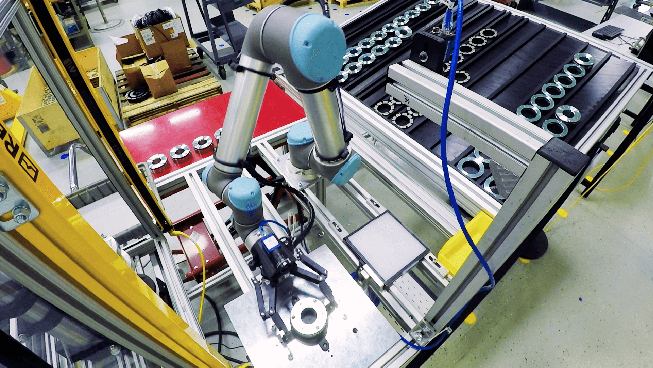
\includegraphics[width=0.75\textwidth]{app1.png}
    \caption{机械臂在工业生产线上}
    \label{fig:tensorboard-success-rate}
\end{figure}

在传统控制框架中，机械臂操作通常由感知、规划和控制等模块组成。系统首先估计目标物体的位置与姿态，然后通过运动规划器生成无碰撞轨迹，最后由底层控制器跟踪轨迹。这类方法结构清晰、可解释性较好，在工业生产线上被广泛应用。然而，传统方法往往依赖较准确的物体模型、环境地图和机械臂标定结果。当物体发生遮挡、堆叠、轻微滑移或接触状态改变时，离线规划得到的轨迹可能不再适用。视觉伺服研究强调利用视觉反馈形成闭环控制\cite{hutchinson1996visualservo,chaumette2006visualservo}，采样式路径规划研究则为高维机械臂空间中的可行路径搜索提供了经典工具\cite{lavalle2001randomized,karaman2011sampling}。但是，在动态目标、障碍物、密集堆叠物体和服务场景长序列任务中，系统仍然需要更强的自主感知与决策能力。

强化学习为机械臂操作提供了一种不同的建模思路。其核心思想是把机器人看作一个智能体，通过与环境交互获得奖励信号，并优化能够最大化长期收益的策略。近年来，深度强化学习在机器人控制、灵巧手操作等任务中取得了显著进展\cite{mnih2015human,openai2019dactyl}。对于机械臂而言，强化学习能够直接从状态和奖励中学习控制策略，减少对人工轨迹设计的依赖，并允许策略在大量仿真交互中逐渐获得“接近目标、形成接触、闭合夹爪、抬升物体、保持稳定”等连续操作能力。与单纯路径规划相比，强化学习更适合描述动作与接触反馈之间的闭环关系；与纯规则控制相比，强化学习能够在一定范围内适应初始状态扰动和物体位姿变化。

与此同时，强化学习在机械臂任务中的应用仍面临训练样本需求大、奖励设计困难、训练过程不稳定、仿真到真实迁移存在差异等问题。相关研究常通过视觉伺服、路径规划、推抓协同、迁移学习和任务知识建模等方式增强策略学习能力。例如，视觉伺服可以提高机械臂对目标相对位姿变化的响应能力；路径规划可以为强化学习提供安全引导；推抓协同可以解决密集堆叠环境中无可行抓取位姿的问题\cite{zeng2018synergies}；迁移学习、多任务基准和目标条件学习可以减少新任务的训练时间并提高泛化能力\cite{andrychowicz2017hindsight,yu2020metaworld}。这些工作表明，机械臂强化学习研究的重点正在从“能否完成任务”进一步转向“是否高效、安全、稳定并可迁移地完成任务”。

本文以桌面物体抬升任务为研究对象。该任务包含机械臂接近、对准、闭合夹爪、接触抓取、抬升和稳定保持等基本操作环节，是研究机械臂强化学习控制的典型任务。本文首先通过仿真平台训练策略，并重点关注策略行为的稳定性，而不是仅关注能否短暂抬起物体；随后将训练得到的策略迁移到 Franka Research 3 真实机械臂平台。选择该任务的意义在于：一方面，它能够用较低的系统复杂度验证强化学习在连续机械臂控制中的有效性；另一方面，抬升后的稳定保持要求与真实机械臂部署中的安全需求密切相关。通过完成从仿真训练到真实机械臂初步验证的闭环流程，本文进一步检验了低维位姿策略在真实平台上的可迁移性和工程实现可行性。

\section{国内外研究现状}

强化学习的基本理论可以追溯到马尔可夫决策过程和动态规划。Sutton 和 Barto 系统总结了强化学习中的价值函数、策略优化、时序差分学习等基础方法\cite{sutton2018reinforcement}。随着深度神经网络的发展，深度强化学习能够处理高维状态和复杂函数逼近问题。DQN 使用深度网络近似动作价值函数，在离散动作控制中取得突破\cite{mnih2015human}。连续控制任务则更适合使用策略梯度、Actor-Critic等方法。机械臂操作属于典型的连续控制问题，策略输出通常对应末端位移、末端速度、关节速度或夹爪开合量，因此需要能够处理连续动作空间的强化学习算法。

从算法角度看，PPO\cite{schulman2017ppo}、DDPG\cite{lillicrap2015ddpg}、TD3 和 SAC 等方法都被广泛用于连续控制任务。其中，SAC 通过最大熵目标鼓励策略保持一定随机性，能够提升探索能力和训练稳定性\cite{haarnoja2018sac}。由于机械臂操作任务常常存在稀疏成功信号和复杂接触状态，SAC 的离策略样本复用能力有助于提高训练效率。近年来，面向机器人操作的研究还进一步关注价值估计偏差、样本效率和多任务泛化问题。例如，Hindsight Experience Replay 通过重新标记目标缓解稀疏奖励问题\cite{andrychowicz2017hindsight}，Meta-World 等基准推动了多任务和元强化学习在机器人操作中的系统评估\cite{yu2020metaworld}。这说明在机器人操作问题中，单一强化学习算法往往需要结合任务结构和先验知识进行改进。

从感知与抓取角度看，视觉信息是机械臂在非结构化环境中完成物体操作的重要来源。早期视觉伺服研究系统讨论了图像特征、相机模型和机器人控制之间的关系，为基于视觉反馈的闭环操作奠定了基础\cite{hutchinson1996visualservo,chaumette2006visualservo}。随着深度学习发展，YOLO 等目标检测方法显著提升了实时物体识别能力\cite{redmon2016yolo}，Lenz 等人使用深度学习检测机器人抓取位姿\cite{lenz2015deep}，Morrison 等人提出的 GGCNN 能够从深度图中实时生成抓取姿态\cite{morrison2018closing}。这类研究表明，强化学习并不是孤立地替代传统控制，而是可以与视觉感知、抓取位姿估计、坐标变换和运动学建模共同构成闭环操作系统。

从路径规划与安全角度看，机械臂在复杂环境中不仅要接近目标，还必须避免碰撞。RRT 和 RRT-Connect 能够在高维空间中快速搜索可行路径\cite{lavalle2001randomized,kuffner2000rrtconnect}，RRT* 进一步给出了渐近最优性分析\cite{karaman2011sampling}。但采样式规划对环境建模和碰撞检测依赖较强，在动态接触任务中仍需与反馈控制或学习方法结合。DQN、Double DQN 和优先经验回放等深度强化学习方法则从价值学习角度提升了智能体在复杂状态空间中的决策能力\cite{mnih2015human,vanhasselt2016deep,schaul2015prioritized}。这类工作对本文具有启发意义：机械臂强化学习的奖励不应只关注终点是否到达，也应关注运动过程是否平稳、安全和可执行。

从复杂物体操作角度看，仅依靠直接抓取并不能覆盖所有场景。在生活和仓储环境中，物体常常密集堆叠或相互遮挡，机器人可能无法直接获得合适抓取位姿。QT-Opt 利用大规模自监督数据训练机器人抓取策略，展示了深度强化学习在真实机器人抓取中的潜力\cite{kalashnikov2018qtopt}；Zeng 等人提出视觉推动与抓取协同学习方法，使机器人能够通过推动改变场景结构，再执行更可靠的抓取\cite{zeng2018synergies}。这些研究说明，机械臂操作算法的发展趋势是从单一动作扩展到多技能协同，并逐步强调泛化性、样本效率和真实环境可用性。

机器人强化学习高度依赖仿真环境。MuJoCo 是常用的机器人动力学仿真引擎，能够提供高效的刚体动力学和接触求解能力\cite{todorov2012mujoco}。robosuite 在 MuJoCo 之上封装了机械臂模型、夹爪模型、桌面操作任务、控制器和传感器接口，为可复现实验提供了便利\cite{zhu2020robosuite}。本文采用 robosuite 中的 Lift 任务作为基础环境，并在其外部构建符合 Gymnasium 接口的强化学习训练包装器。面向单物体抬升任务训练强化学习控制策略，使机械臂在完成接近和夹取后，能够将物体抬升到目标高度附近并保持静止，保证了强化学习策略从仿真走向真实机械臂时的稳定性与安全性。

\section{本文主要工作}

本文的主要工作包括以下几个方面：

\begin{enumerate}
  \item 基于 robosuite 和 MuJoCo 搭建机械臂桌面立方体抬升仿真环境，选用 Franka Panda / Franka Research 3 机械臂和操作空间位置控制器作为实验平台。
  \item 设计低维状态空间，将末端位置、夹爪开合量、立方体位置、立方体四元数以及末端到立方体的相对位置组合为策略输入，降低视觉训练的复杂度。
  \item 使用 SAC 算法训练连续动作控制策略，并通过 TensorBoard 记录奖励、成功率、回合长度等指标。
  \item 针对训练策略中出现的过度上抬和随机摆动问题，设计稳定抬升奖励、动作惩罚、速度惩罚和连续保持成功判据。
  \item 面向 Franka Research 3 真实机械臂完成初步 sim-to-real 验证。真实系统使用 RealSense 相机和 ArUco 标记估计立方体位姿，通过手眼标定将相机坐标系下的物体位姿转换到机器人基坐标系，并构造与仿真一致的低维观测，加载训练得到的最优策略模型进行推理。真实执行阶段将策略输出的归一化位置动作转换为受限的笛卡尔线性位移，并根据策略第四维动作控制 Franka Hand 闭合，从而完成真实平台上的接近、夹取和抬升验证。

\begin{figure}[htbp]
    \centering
    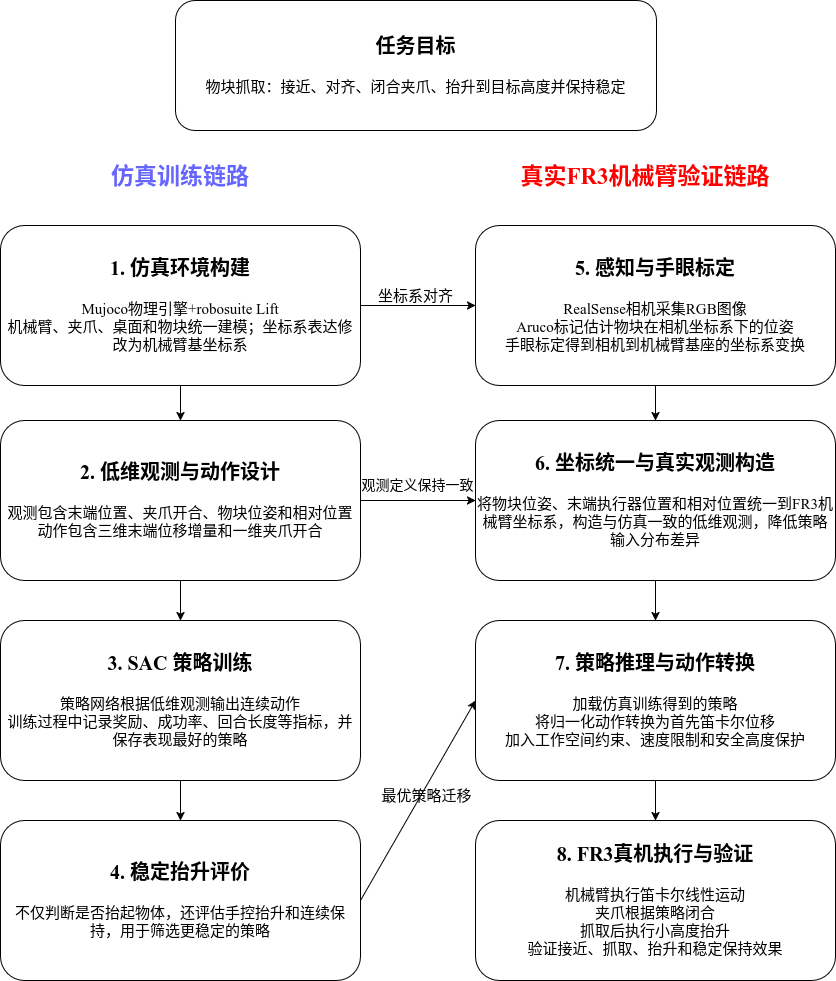
\includegraphics[width=1.0\textwidth]{frame.png}
    \caption{仿真实验到真机验证的方法框架}
    \label{fig:sim-to-real-method-framework}
\end{figure}

\end{enumerate}

\section{论文结构}

本文共分为六章。第一章介绍研究背景、研究现状和主要工作。第二章介绍机械臂控制与强化学习相关理论。第三章描述系统环境、状态动作空间、训练流程以及稳定抬升控制方法。第四章给出实验设计与结果分析。第五章讨论真实机械臂部署方案与安全约束。第六章总结全文。

\chapter{相关理论基础}

\section{机械臂运动控制基础}

机械臂通常由多个转动或移动关节串联组成。对于串联机械臂而言，关节空间描述的是各关节的位置、速度和力矩，任务空间描述的是末端执行器在三维空间中的位置和姿态。机械臂控制算法的核心问题之一，就是建立关节空间与任务空间之间的映射关系，并在满足关节限位、速度限制和碰撞约束的条件下，使末端执行器完成预期操作。

设机械臂关节变量为
\begin{equation}
  \boldsymbol{q} = [q_1, q_2, \dots, q_n]^T,
\end{equation}
其中 $n$ 为自由度数量。末端执行器在笛卡尔空间中的位姿可表示为
\begin{equation}
  \boldsymbol{x} = f(\boldsymbol{q}),
\end{equation}
其中 $f(\cdot)$ 为正运动学映射。末端速度与关节速度之间满足
\begin{equation}
  \dot{\boldsymbol{x}} = \boldsymbol{J}(\boldsymbol{q})\dot{\boldsymbol{q}},
\end{equation}
其中 $\boldsymbol{J}(\boldsymbol{q})$ 为雅可比矩阵。

雅可比矩阵不仅用于速度映射，也用于把任务空间误差转换为关节空间控制量。当机械臂接近奇异位形时，雅可比矩阵可能出现秩亏，导致某些方向上的末端速度难以通过有限关节速度实现。因此，在真实机械臂控制中，通常需要结合速度限制、阻尼伪逆、关节限位规避和工作空间约束等策略，避免机械臂进入不稳定或不可控区域。

机械臂动力学可用如下形式表示：
\begin{equation}
  \boldsymbol{M}(\boldsymbol{q})\ddot{\boldsymbol{q}}
  + \boldsymbol{C}(\boldsymbol{q},\dot{\boldsymbol{q}})\dot{\boldsymbol{q}}
  + \boldsymbol{g}(\boldsymbol{q})
  = \boldsymbol{\tau} + \boldsymbol{J}^T(\boldsymbol{q})\boldsymbol{F},
\end{equation}
其中 $\boldsymbol{M}$ 为惯性矩阵，$\boldsymbol{C}$ 为科氏力和离心力项，$\boldsymbol{g}$ 为重力项，$\boldsymbol{\tau}$ 为关节力矩，$\boldsymbol{F}$ 为末端外力。对于包含接触的操作任务，末端力和物体接触状态会影响机械臂运动，因此纯位置轨迹跟踪往往不足以描述完整任务。

在桌面抓取任务中，直接控制关节角度虽然可行，但策略需要学习从任务空间目标到关节空间动作的复杂映射。为了降低学习难度，本文采用操作空间控制（Operational Space Control, OSC）作为底层控制方式\cite{khatib1987osc}。在该方式下，强化学习策略输出末端执行器在三维空间中的小位移，底层控制器负责将末端目标转换为关节力矩或关节控制命令。这样可以让策略更直接地关注“末端应该向哪里移动”。

操作空间控制通常在任务空间中定义末端误差：
\begin{equation}
  \boldsymbol{e}_x = \boldsymbol{x}_{d} - \boldsymbol{x},
\end{equation}
其中 $\boldsymbol{x}_{d}$ 为期望末端位姿，$\boldsymbol{x}$ 为当前末端位姿。控制器根据末端误差、末端速度以及机械臂动力学模型生成关节控制量。对于本文使用的 OSC\_POSITION 控制器，策略不直接输出姿态变化，而是输出末端位置增量和夹爪动作。该设计减少了动作空间维度，有利于在立方体抬升任务中提高训练效率。

\section{机械臂抓取任务建模}

机械臂抓取任务通常可以分为接近、对准、闭合夹爪、形成稳定接触、抬升和放置等阶段。不同阶段的控制目标并不完全相同：接近阶段强调末端与目标物体之间的相对位置误差；抓取阶段强调夹爪与物体表面的接触关系；抬升阶段则要求物体随夹爪稳定运动，并避免过大的速度、加速度和摆动。

对于平行夹爪或二指夹爪，抓取是否成功不仅取决于末端位置，还取决于夹爪开合宽度、接触点、摩擦条件和物体质心位置。若夹爪闭合时物体未处于合适区域，可能出现夹空、碰撞、推开物体或抓取后滑落等现象。因此，强化学习环境中的状态设计需要尽量包含与任务成功相关的信息。本文采用低维观测，包括末端位置、夹爪开合量、立方体位姿和末端到立方体的相对位置，正是为了让策略能够根据几何关系学习接近和抬升动作。

机械臂操作任务中的动作空间通常有三种设计方式。第一种是关节空间动作，即策略直接输出关节位置、速度或力矩；第二种是任务空间动作，即策略输出末端位置、速度或姿态增量；第三种是高层动作，即策略输出抓取点、目标位姿或技能参数，再由运动规划器和控制器执行。关节空间动作表达能力强，但学习难度较高；任务空间动作更接近人类对抓取任务的描述，适合桌面操作；高层动作安全性较好，但依赖额外规划模块。本文选用任务空间位置增量作为动作，兼顾了学习难度和控制直观性。

抓取任务奖励函数一般包含稀疏奖励和稠密奖励两类。稀疏奖励只在任务成功时给出正奖励，定义清晰但探索困难；稠密奖励会在接近目标、夹住物体、抬升物体等中间阶段给出反馈，能够提高训练效率，但也可能引入策略投机行为。例如，若奖励只鼓励物体高度增加，策略可能学会过度上抬或在成功后继续摆动。本文后续设计稳定抬升奖励和连续保持成功判据，就是为了解决原始奖励与期望行为不完全一致的问题。

\section{马尔可夫决策过程}

强化学习关注智能体如何通过与环境交互来学习决策策略。在机械臂操作任务中，机械臂及其控制策略可视为智能体，仿真或真实操作场景可视为环境。智能体在每一个控制时刻根据当前观测选择动作，动作作用于环境后，环境状态发生变化，并返回奖励信号。奖励用于评价当前动作对任务目标的贡献，智能体则根据奖励不断更新策略参数，最终学习到能够获得较高长期回报的行为方式。

\begin{figure}[htbp]
    \centering
    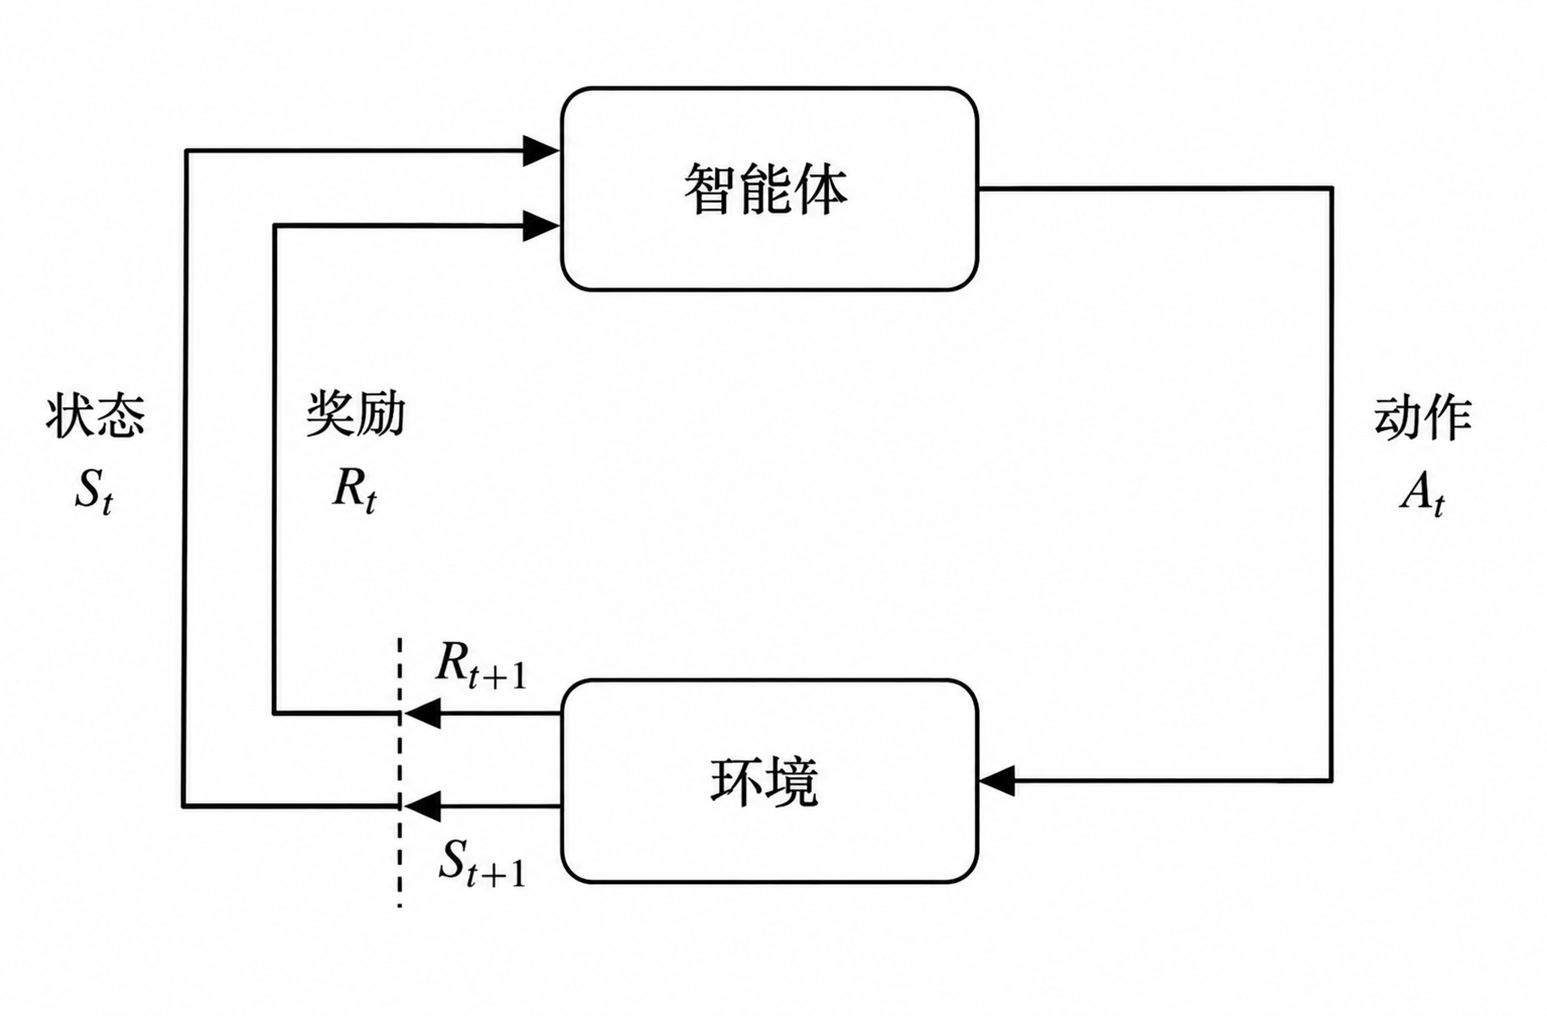
\includegraphics[width=0.75\textwidth]{rl-agent-env.png}
    \caption{强化学习智能体-环境交互原理图}
    \label{fig:tensorboard-success-rate}
\end{figure}

以本文的立方体抬升任务为例，机械臂在某一时刻观测到末端位置、夹爪状态和立方体位置后，策略输出末端位移和夹爪动作。环境执行该动作后，立方体位置、末端位置和夹爪状态发生变化，同时根据机械臂是否接近物体、是否抓住物体、是否稳定抬升等条件返回奖励。如此循环进行，便构成了强化学习中的交互过程。

% 图示占位：此处可添加“强化学习智能体-环境交互原理图”，类似：状态 s_t -> 智能体 -> 动作 a_t -> 环境 -> 奖励 r_t 和下一状态 s_{t+1}。

强化学习问题通常建模为马尔可夫决策过程。一个马尔可夫决策过程可表示为五元组
\begin{equation}
  \mathcal{M} = (\mathcal{S}, \mathcal{A}, P, r, \gamma),
\end{equation}
其中 $\mathcal{S}$ 为状态空间，$\mathcal{A}$ 为动作空间，$P$ 为状态转移函数，$r$ 为奖励函数，$\gamma \in [0,1)$ 为折扣因子。状态转移函数表示智能体在状态 $s$ 下执行动作 $a$ 后转移到下一状态 $s'$ 的概率：
\begin{equation}
  P_{ss'}^{a}=P(s_{t+1}=s'|s_t=s,a_t=a).
\end{equation}
奖励函数表示智能体在状态 $s$ 下执行动作 $a$ 后所获得的期望反馈：
\begin{equation}
  R_s^a=\mathbb{E}(r_{t+1}|s_t=s,a_t=a).
\end{equation}
折扣因子 $\gamma$ 用于平衡近期奖励和远期奖励。当 $\gamma$ 较小时，智能体更关注短期收益；当 $\gamma$ 较大时，智能体更重视长期结果。在机械臂抓取任务中，若只关注短期奖励，策略可能只学习到快速接近物体；若考虑长期奖励，策略才会倾向于完成接近、夹取、抬升和保持稳定的完整过程。

策略函数描述智能体在状态下选择动作的行为准则，通常记为
\begin{equation}
  \pi(a|s)=P(a_t=a|s_t=s).
\end{equation}
对于确定性策略，状态会直接映射到一个动作；对于随机策略，状态会映射到动作概率分布。SAC 属于随机策略方法，其策略网络输出动作分布，并从中采样动作执行。

从某一时刻开始，智能体未来能够获得的折扣累积回报定义为
\begin{equation}
  G_t=r_{t+1}+\gamma r_{t+2}+\gamma^2 r_{t+3}+\cdots
  =\sum_{k=0}^{\infty}\gamma^k r_{t+k+1}.
\end{equation}
强化学习的目标是学习策略 $\pi(a|s)$，使期望折扣回报最大：
\begin{equation}
  J(\pi)=\mathbb{E}_{\pi}\left[\sum_{t=0}^{T}\gamma^t r(s_t,a_t)\right].
\end{equation}

对于机械臂操作任务，状态可以由机器人本体状态和物体状态组成，动作可以是关节控制量、末端速度或末端位移。奖励函数则用于刻画任务目标，例如接近物体、成功抓取、抬升物体和保持稳定等。

在实际机器人任务中，环境往往并不完全满足完全可观测假设。真实系统中可能存在视觉遮挡、传感器噪声、物体姿态估计误差和控制延迟等问题，此时智能体获得的观测 $o_t$ 只是状态 $s_t$ 的一部分。该问题更严格地说可以建模为部分可观测马尔可夫决策过程。本文在仿真阶段直接使用低维状态观测，因此暂不引入循环神经网络或历史观测编码。但为了缓解单帧观测缺少速度信息的问题，本文在稳定判据中额外计算立方体速度和末端速度，并在奖励中加入运动惩罚。

强化学习中的价值函数用于评价状态或状态动作对的长期收益。状态价值函数定义为
\begin{equation}
  V^{\pi}(s)=\mathbb{E}_{\pi}\left[\sum_{t=0}^{T}\gamma^t r_t \mid s_0=s\right],
\end{equation}
动作价值函数定义为
\begin{equation}
  Q^{\pi}(s,a)=\mathbb{E}_{\pi}\left[\sum_{t=0}^{T}\gamma^t r_t \mid s_0=s,a_0=a\right].
\end{equation}
最优策略 $\pi^*$ 是使所有状态下价值函数达到最大的策略，可表示为
\begin{equation}
  \pi^*=\arg\max_{\pi} V^{\pi}(s).
\end{equation}
若使用动作价值函数进行动作选择，则最优动作可由
\begin{equation}
  a^*=\arg\max_a Q^*(s,a)
\end{equation}
得到。基于价值的方法通过估计 $Q$ 函数选择高价值动作，基于策略的方法直接优化策略参数，Actor-Critic方法则同时学习策略和价值函数。机械臂连续控制任务中动作维度连续，难以像离散动作任务那样枚举所有动作，因此Actor-Critic结构被广泛使用。

随着深度神经网络的发展，价值函数和策略函数可以由神经网络近似表示。状态向量作为网络输入，网络输出动作、动作分布或价值估计。对于本文使用的低维状态，网络不需要处理图像特征，因而可以采用多层感知机结构。这种设计减少了训练复杂度，使实验重点集中在连续控制策略和稳定抬升奖励设计上。

\section{连续控制强化学习算法}

机械臂控制中的动作通常是连续变量，因此连续控制算法是机器人强化学习的重要基础。DDPG 将确定性策略梯度与深度 Q 网络结合，能够在连续动作空间中进行离策略学习\cite{lillicrap2015ddpg}。但 DDPG 对超参数、探索噪声和价值估计误差较为敏感。TD3 在 DDPG 基础上引入双Critic网络、目标策略平滑和延迟策略更新，以缓解 Q 值过估计问题\cite{fujimoto2018td3}。PPO 则通过限制新旧策略更新幅度提高训练稳定性，属于常用的在线策略优化方法\cite{schulman2017ppo}。

与上述方法相比，SAC 在目标函数中显式引入策略熵，使策略既追求高回报，也保持一定随机性。对于机械臂任务而言，这一点具有实际意义：训练早期策略需要探索不同接近方向、夹爪开合时机和抬升动作；训练后期则需要逐渐收敛到稳定可靠的动作模式。最大熵强化学习能够在探索和利用之间取得较好的平衡。

在选择具体算法时，需要考虑样本效率、训练稳定性、动作空间类型和实现复杂度。本文任务使用仿真环境训练，能够生成较多交互样本，但接触任务仍存在奖励噪声和策略不稳定问题。因此本文选用 SAC 作为主要算法，并使用 Stable-Baselines3 中经过工程验证的实现，降低算法实现错误对实验结果的影响。

\section{Soft Actor-Critic（SAC）算法}

SAC 是一种离策略Actor-Critic算法，其核心特点是在最大化任务回报的同时最大化策略熵，从而鼓励策略探索。Actor-Critic 结构由策略网络和价值网络组成。策略网络也称为 Actor，负责根据状态输出动作分布；价值网络也称为 Critic，负责评价当前状态动作对的价值，并为 Actor 的参数更新提供方向。相比只学习价值函数的方法，Actor-Critic 更适合连续动作空间；相比只使用策略梯度的方法，Critic 能够降低策略更新方差，提高训练效率。

% 图示占位：此处可添加“SAC 网络结构图”，建议包括 Actor、两个 Critic、两个 Target Critic、Replay Buffer 以及环境交互箭头。

SAC 的最大熵目标函数可写为
\begin{equation}
  J(\pi)=\sum_{t=0}^{T}\mathbb{E}_{(s_t,a_t)\sim\rho_{\pi}}
  \left[r(s_t,a_t)+\alpha\mathcal{H}(\pi(\cdot|s_t))\right],
\end{equation}
其中 $\alpha$ 为熵温度系数，$\mathcal{H}$ 表示策略熵。策略熵定义为
\begin{equation}
  \mathcal{H}(\pi(\cdot|s))=
  \mathbb{E}_{a\sim\pi}\left[-\log \pi(a|s)\right].
\end{equation}
熵越大，说明策略在多个动作之间分布更均匀，探索性更强；熵越小，说明策略更倾向于选择少数高价值动作，利用性更强。较大的熵鼓励策略在训练早期保持随机探索，较小的熵则使策略在任务收敛后更加确定。

SAC 通常包含一个 Actor 网络、两个 Critic 网络、两个 Target Critic 网络以及经验回放池。设置两个 Critic 网络的目的是缓解价值函数过估计问题；Target Critic 网络用于构造相对稳定的训练目标；经验回放池用于保存历史交互样本。训练时，算法从回放池中随机抽取 $(s_t,a_t,r_t,s_{t+1})$ 样本，分别更新 Critic、Actor 和温度系数。

SAC 的软 Q 函数更新目标可表示为
\begin{equation}
  y = r + \gamma \left( \min_{i=1,2} Q_{\bar{\theta}_i}(s',a')
  - \alpha \log \pi_{\phi}(a'|s') \right),
\end{equation}
其中 $Q_{\bar{\theta}_i}$ 为目标 Q 网络，$a'$ 由当前策略在下一状态 $s'$ 下采样得到。使用两个 Q 网络并取较小值，可以减轻价值函数过估计问题。策略网络的优化目标为
\begin{equation}
  J_{\pi}(\phi)=
  \mathbb{E}_{s\sim \mathcal{D}, a\sim\pi_{\phi}}
  \left[\alpha \log \pi_{\phi}(a|s)-\min_{i=1,2}Q_{\theta_i}(s,a)\right],
\end{equation}
其中 $\mathcal{D}$ 为经验回放池。该目标鼓励策略选择高 Q 值动作，同时通过熵项保持探索。

温度系数 $\alpha$ 控制熵项权重。当 $\alpha$ 较大时，策略更随机，探索更充分；当 $\alpha$ 较小时，策略更倾向于选择当前估计价值较高的动作。实际训练中常使用自动熵系数调整，使策略熵接近目标熵。本文实验采用自动温度调节方式，使策略能够在探索和利用之间保持较好的平衡。

SAC 的离策略特性使其可以从历史数据中反复采样训练，这对机械臂仿真任务较为重要。机械臂每一步仿真都需要进行动力学计算和接触求解，采样成本高于普通数值环境。经验回放能够提高样本利用率，使相同交互数据多次参与网络更新。与此同时，回放池也会混合早期低质量数据和后期高质量数据，因此学习率、批大小、回放池大小和起始学习步数都会影响训练稳定性。

% 建议步骤：
% 1. 初始化 Actor、两个 Critic、两个 Target Critic 和 Replay Buffer；
% 2. 与环境交互并存储 (s_t, a_t, r_t, s_{t+1})；
% 3. 从 Replay Buffer 采样 mini-batch；
% 4. 根据软 Bellman 目标更新 Critic；
% 5. 根据最大熵目标更新 Actor；
% 6. 自动调整温度系数 alpha；
% 7. 软更新 Target Critic。
\begin{table}[htbp]
  \centering
  \caption{SAC 算法训练流程}
  \label{alg:sac-training}
  \begin{tabular}{p{0.92\textwidth}}
    \toprule
    \textbf{输入：}环境 $\mathcal{E}$，折扣因子 $\gamma$，软更新系数 $\tau$，批大小 $B$，目标熵 $\mathcal{H}_{target}$。\\
    \textbf{初始化：}Actor 网络 $\pi_{\phi}$，两个 Critic 网络 $Q_{\theta_1},Q_{\theta_2}$，两个 Target Critic 网络 $Q_{\bar{\theta}_1},Q_{\bar{\theta}_2}$，经验回放池 $\mathcal{D}$，温度系数 $\alpha$。\\
    \midrule
    1. \textbf{for} 每一个训练回合 \textbf{do}\\
    \quad 2. 重置环境，获得初始状态 $s_0$；\\
    \quad 3. \textbf{for} 每一个控制步 $t$ \textbf{do}\\
    \quad\quad 4. 根据当前策略采样动作 $a_t \sim \pi_{\phi}(\cdot|s_t)$；\\
    \quad\quad 5. 在环境中执行 $a_t$，获得奖励 $r_t$ 和下一状态 $s_{t+1}$；\\
    \quad\quad 6. 将转移样本 $(s_t,a_t,r_t,s_{t+1})$ 存入经验回放池 $\mathcal{D}$；\\
    \quad\quad 7. 从 $\mathcal{D}$ 中采样 mini-batch，样本数量为 $B$；\\
    \quad\quad 8. 对每个样本，根据当前 Actor 在 $s_{t+1}$ 处采样下一动作 $a'$；\\
    \quad\quad 9. 计算软 Bellman 目标
    $
      y=r_t+\gamma\left(\min_{i=1,2}Q_{\bar{\theta}_i}(s_{t+1},a')-\alpha\log\pi_{\phi}(a'|s_{t+1})\right)
    $；\\
    \quad\quad 10. 最小化 $\left(Q_{\theta_i}(s_t,a_t)-y\right)^2$，更新两个 Critic 网络；\\
    \quad\quad 11. 最小化
    $
      \alpha\log\pi_{\phi}(a|s_t)-\min_{i=1,2}Q_{\theta_i}(s_t,a)
    $，更新 Actor 网络；\\
    \quad\quad 12. 根据目标熵 $\mathcal{H}_{target}$ 自动调整温度系数 $\alpha$；\\
    \quad\quad 13. 软更新目标网络：
    $
      \bar{\theta}_i \leftarrow \tau\theta_i+(1-\tau)\bar{\theta}_i
    $；\\
    \quad\quad 14. 令 $s_t \leftarrow s_{t+1}$；\\
    \quad 15. \textbf{end for}\\
    16. \textbf{end for}\\
    \textbf{输出：}训练后的策略网络 $\pi_{\phi}$。\\
    \bottomrule
  \end{tabular}
\end{table}

\section{奖励函数与评价指标}

奖励函数是强化学习任务设计的核心。对于机械臂操作任务，奖励函数既要表达最终目标，也要引导策略学习合理的中间行为。若奖励过于稀疏，策略可能很难通过随机探索发现成功动作；若奖励过于复杂，策略可能利用奖励漏洞形成不符合实际需求的行为。因此，奖励设计需要在学习效率和目标一致性之间取得平衡。

本文任务的原始目标是将立方体抬离桌面。robosuite 的 Lift 环境提供了 shaped reward，用于鼓励末端接近物体和抓取物体。但在实际训练观察中，仅用原始成功条件会出现策略抬起后继续上升或随机摆动的问题。这说明“物体高度超过阈值”并不等价于“稳定完成抬升”。因此，本文进一步引入目标抬升高度、物体速度、末端速度、动作幅值和连续保持步数等指标。

本文将评价指标分为三个层次。第一层为 raw\_lift\_success，表示立方体是否达到 robosuite 原始抬升成功阈值；第二层为 controlled\_lift，表示立方体是否处于目标高度附近且运动速度较小；第三层为 held\_success，表示 controlled\_lift 状态是否连续保持若干控制步。分层指标能够区分“短暂抬起”“受控抬起”和“稳定保持”，比单一成功率更适合评价真实机械臂部署前的策略质量。

\section{手眼标定}

在仿真环境中，机械臂末端位姿和物体位姿可以直接从 MuJoCo 状态中读取，并且二者天然处于同一个仿真世界坐标系下。但在真实机械臂系统中，物体位姿通常由外部相机检测得到，机械臂末端位姿则由机器人正运动学或 TF 系统给出。若相机坐标系和机器人基坐标系之间的空间关系未知，则无法正确计算末端到物体的相对位置，也无法构造与仿真一致的策略观测。因此，sim-to-real 部署的关键步骤之一就是进行手眼标定，建立相机坐标系与机器人基坐标系之间的刚体变换。

手眼标定的目标是求解相机坐标系与机器人坐标系之间的外参。根据相机安装方式不同，常见形式包括 eye-in-hand 和 eye-on-base。eye-in-hand 表示相机安装在机械臂末端，随着机械臂运动而运动；eye-on-base 表示相机固定在环境或机器人基座附近，相机相对于机器人基坐标系保持不变。本文真实系统采用 eye-on-base 方式，即 RealSense 相机固定在工作空间外部，标定目标是求解机器人基坐标系到相机标定光学坐标系的变换。

齐次变换矩阵可以表示一个坐标系相对于另一个坐标系的位姿：
\begin{equation}
  {}^{A}T_{B}
  =
  \begin{bmatrix}
    {}^{A}R_{B} & {}^{A}\boldsymbol{t}_{B} \\
    \boldsymbol{0}^{T} & 1
  \end{bmatrix},
\end{equation}
其中 ${}^{A}R_{B}$ 为坐标系 $B$ 到坐标系 $A$ 的旋转矩阵，${}^{A}\boldsymbol{t}_{B}$ 为坐标系 $B$ 原点在坐标系 $A$ 下的位置。对于真实抓取任务，若视觉检测得到物体相对于相机的变换 ${}^{camera}T_{cube}$，手眼标定得到相机相对于机器人基坐标系的变换 ${}^{base}T_{camera}$，则物体在机器人基坐标系下的位姿为
\begin{equation}
  {}^{base}T_{cube}
  =
  {}^{base}T_{camera}
  {}^{camera}T_{cube}.
\end{equation}
该式是将视觉检测结果用于真实机器人控制的基础。只有得到 ${}^{base}T_{cube}$ 后，才能与机器人正运动学给出的末端位姿 ${}^{base}T_{eef}$ 在同一坐标系下计算相对位置。

对于本文使用的低维策略，真实观测中需要计算
\begin{equation}
  \boldsymbol{p}_{rel}
  =
  \boldsymbol{p}_{cube}^{base}
  -
  \boldsymbol{p}_{eef}^{base}.
\end{equation}
该相对位置必须在机器人基坐标系下计算。如果直接使用相机坐标系下的 \(\boldsymbol{p}_{cube}^{camera}\)，则其 $x$、$y$、$z$ 轴方向与机器人基坐标系不同，原点也不一致，策略会把错误的空间方向解释为末端运动方向，从而导致真实机械臂向错误方向移动。因此，手眼标定不仅是视觉系统的准备步骤，也是保持仿真观测和真实观测一致性的必要条件。

手眼标定通常通过让机器人末端或标定板在多个不同位姿下运动，并同时记录机器人位姿和相机观测位姿来求解。以 eye-on-base 标定为例，机器人基坐标系到末端的变换 ${}^{base}T_{eef}$ 可由机器人正运动学获得，相机到标定板或标记的变换 ${}^{camera}T_{marker}$ 可由视觉检测获得。通过多组不同姿态下的对应关系，可以估计固定不变的 ${}^{base}T_{camera}$。标定完成后，该外参可作为静态变换发布，使系统能够自动完成机器人基坐标系、相机坐标系、物体坐标系和末端坐标系之间的变换查询。

% 图示占位：此处可添加“手眼标定原理图”，展示 fr3_link0、camera_calib_optical_frame、marker/cube、fr3_hand_tcp 之间的齐次变换关系。
\begin{figure}[htbp]
    \centering
    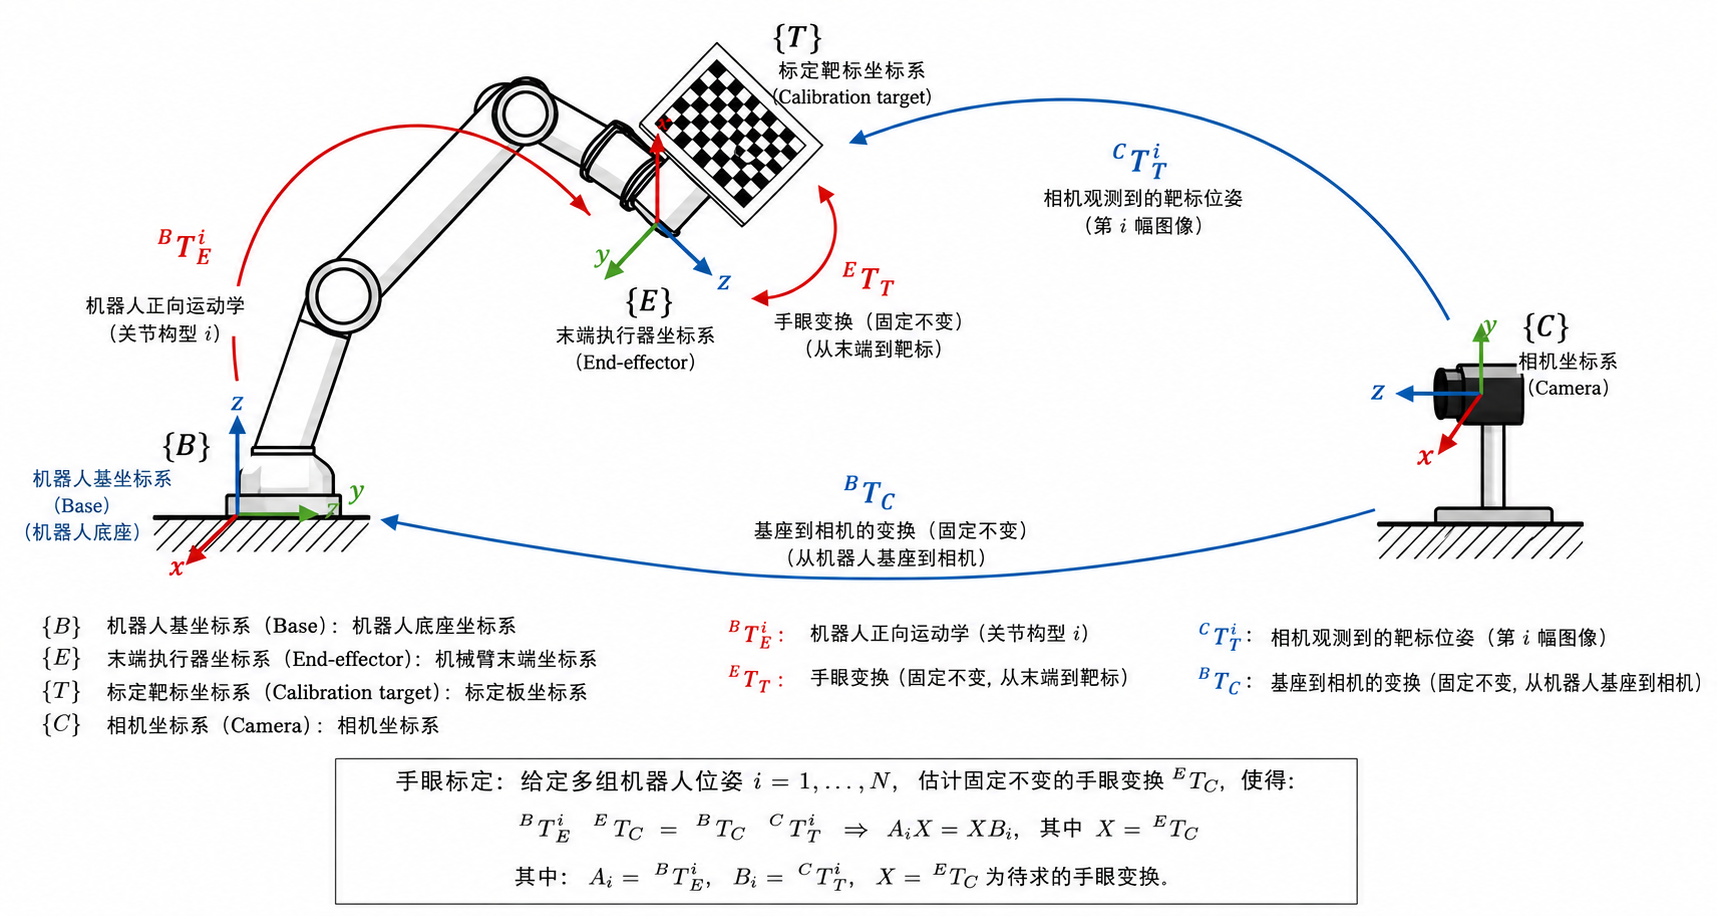
\includegraphics[width=1.0\textwidth]{hand-eye-calib.png}
    \caption{手眼标定原理图}
    \label{fig:tensorboard-success-rate}
\end{figure}

在真实部署中，手眼标定结果还需要通过实际测量和坐标查询进行验证。常用检查方式包括：观察立方体在机器人基坐标系下的位置是否落在真实桌面任务区域内；移动立方体时，物体位置变化方向是否与机器人基坐标系方向一致；查询末端 TCP 位姿是否与机器人实际姿态一致。只有这些检查通过后，强化学习策略才能安全地使用真实观测进行推理。

\chapter{系统设计与实现}

\section{总体架构}

本文实现的机械臂强化学习系统由四个部分组成：仿真环境、Gymnasium 包装器、强化学习算法和实验记录模块。仿真环境由 robosuite 创建，负责 MuJoCo 模型加载、物理仿真、奖励计算和观测生成；包装器负责将 robosuite 的字典观测转换为低维向量，并对动作进行工作空间约束；强化学习算法采用 Stable-Baselines3 中的 SAC 实现\cite{stablebaselines3}；实验记录模块通过 TensorBoard 保存训练曲线。

从软件实现角度看，系统首先创建 robosuite 的 Lift 任务环境，然后通过自定义环境包装模块将其封装为 Gymnasium 接口。Stable-Baselines3 中的 SAC 算法不直接访问 robosuite 原始环境，而是通过该包装模块读取观测、发送动作并获得奖励。这样做的好处是：一方面保持了 robosuite 物理环境的完整性；另一方面可以在包装层中加入观测降维、动作尺度转换、工作空间裁剪、成功率统计和日志记录等任务相关逻辑。

% 【方法框架图占位 1：仿真训练总体框架图】
% 建议画出 robosuite/MuJoCo 环境、Gymnasium Wrapper、低维观测构造、SAC Agent、动作裁剪与奖励计算、Monitor/EvalCallback、TensorBoard 日志之间的关系。
% 推荐箭头：环境观测 -> Wrapper -> SAC 策略 -> 动作缩放/裁剪 -> 环境执行 -> 奖励与成功率指标 -> 策略更新/日志记录。

系统流程如下：
\begin{enumerate}
  \item 初始化 Lift 环境、Panda 机械臂、Panda 夹爪和 OSC\_POSITION 控制器；
  \item 从环境中读取末端位置、夹爪状态和立方体状态；
  \item 将观测拼接为固定维度向量，输入 SAC 策略网络；
  \item 策略输出连续动作，包括末端位置增量和夹爪动作；
  \item 包装器将动作裁剪到安全工作空间内，并传入 robosuite 环境；
  \item 环境执行控制步，返回新状态、奖励、终止标志和诊断信息；
  \item SAC 使用交互数据更新策略，并定期进行评估。
\end{enumerate}

在该流程中，仿真环境和强化学习算法之间并不是简单直接连接，而是通过包装器进行数据格式转换与安全约束。robosuite 原始观测为字典结构，包含机器人本体状态、物体状态和可选相机图像等多种信息；SAC 算法需要固定维度的向量输入。因此，包装器需要明确选择哪些观测量作为策略输入，并保证每次 reset 和 step 返回的数据维度一致。

\section{仿真环境配置}

本文基于 robosuite 的 Lift 任务开展实验。该任务包含一张桌子、一个立方体物块、一个单臂机械臂和一个二指夹爪。机械臂需要从初始位姿出发，移动到立方体附近，闭合夹爪抓取物体，并将其从桌面上抬起。

环境关键参数如表 \ref{tab:env-config} 所示。

\begin{table}[htbp]
  \centering
  \caption{仿真环境主要参数}
  \label{tab:env-config}
  \begin{tabular}{ll}
    \toprule
    参数 & 取值 \\
    \midrule
    仿真平台 & MuJoCo + robosuite \\
    任务名称 & Lift \\
    机械臂模型 & FR3v2 \\
    控制器 & OSC\_POSITION \\
    控制频率 & 20 Hz \\
    单回合最大步数 & 200 \\
    是否使用图像观测 & 否 \\
    是否使用物体状态观测 & 是 \\
    强化学习算法 & SAC \\
    \bottomrule
  \end{tabular}
\end{table}

在 robosuite 原始 Lift 任务中，当立方体高度超过桌面一定阈值时即判定为成功。该定义适合衡量是否完成“抬起”动作，但无法区分抬起后的稳定性。本文在外部包装器中引入更严格的稳定保持指标。

环境创建时关闭相机图像观测，策略不直接使用图像作为输入；同时保留低维物体状态，使环境能够提供立方体位置、姿态以及末端与立方体之间的相对位置等信息。该设置适合本文当前阶段的算法验证，因为它避免了视觉识别误差对强化学习训练的影响，使研究重点集中在连续控制策略和稳定抬升目标上。

控制器方面，本文使用操作空间位置控制器。该控制器接收末端位置增量，不要求策略直接输出关节角度或关节力矩。对于立方体抬升任务，末端位置控制已经能够表达接近、下降、夹取和上抬等主要动作。与同时控制末端位置和姿态的方式相比，仅控制末端位置的动作维度更低，训练难度更小；与关节控制相比，末端位置动作更符合任务空间直觉。

Lift 环境的单回合最大步数设置为 200，控制频率为 20 Hz，因此一个完整回合对应约 10 s 仿真时间。若策略在回合内达到稳定保持成功条件，包装器可提前终止回合；若未达到成功条件，则回合在 200 步时因时间限制结束。

\section{状态空间设计}

为了降低训练难度，本文不使用图像作为输入，而是使用低维状态观测。单步观测向量维度为 14，具体组成如表 \ref{tab:obs-space} 所示。

\begin{table}[htbp]
  \centering
  \caption{低维观测向量组成}
  \label{tab:obs-space}
  \begin{tabular}{lll}
    \toprule
    索引范围 & 维度 & 含义 \\
    \midrule
    0:3 & 3 & 机械臂末端位置 \\
    3:4 & 1 & 夹爪开合量 \\
    4:7 & 3 & 立方体位置 \\
    7:11 & 4 & 立方体四元数姿态 \\
    11:14 & 3 & 末端到立方体的相对位置 \\
    \bottomrule
  \end{tabular}
\end{table}

该状态设计的优点是维度低、学习效率高，并且能够直接反映抓取任务所需的几何关系。其不足是依赖仿真环境提供的精确物体位姿。在真实机器人部署时，需要通过视觉定位估计物体位姿。

观测向量由环境包装模块生成。该模块从环境返回的观测信息中提取末端位置、夹爪开合量、立方体位置、立方体姿态以及末端到立方体的相对位置，并按固定顺序拼接为一维数组。其中，夹爪原始关节状态被压缩为一维开合量，以减少冗余信息。

状态空间各部分的作用如下：末端位置用于描述机械臂当前执行器位置；夹爪开合量用于判断夹爪是否处于打开、闭合或半闭合状态；立方体位置用于提供目标物体的空间坐标；立方体四元数用于描述物体姿态；末端到立方体的相对位置直接反映抓取任务中最重要的几何误差。相比仅使用末端位置和物体位置，相对位置能够减少神经网络自行学习坐标差的负担。

本文当前没有把速度信息直接加入策略观测，主要原因是希望保持状态维度较低，并先验证位置状态下的抓取能力。速度信息虽然不作为策略输入，但会在稳定抬升判据和奖励函数中使用，用于判断物体和末端是否已经保持稳定。

\section{动作空间设计}

本文采用 OSC\_POSITION 控制器。策略动作向量为 4 维：
\begin{equation}
  \boldsymbol{a}=[a_x,a_y,a_z,a_g]^T,
\end{equation}
其中前三维表示末端执行器在操作空间中的位置增量，最后一维表示夹爪开合控制。动作范围为 $[-1,1]$。需要注意的是，robosuite 暴露给策略的动作是归一化动作，底层控制器会将其映射到实际末端位移范围。因此，在进行工作空间裁剪时，不能直接把归一化动作当作米制位移，而应先转换到控制器实际输出尺度，再进行裁剪。

本文包装器中实现了归一化动作与末端位移之间的双向转换：
\begin{equation}
  \Delta x = \frac{a-a_{\min}}{a_{\max}-a_{\min}}
  (\Delta x_{\max}-\Delta x_{\min})+\Delta x_{\min}.
\end{equation}
这样可以保证工作空间约束与真实几何尺度一致。

具体而言，策略网络输出的前三维动作 $a_x,a_y,a_z$ 位于 $[-1,1]$ 区间内。操作空间控制器内部会将其缩放到实际末端位置增量范围。以默认配置为例，归一化动作 $[-1,1]$ 对应的末端位置增量约为 $[-0.05,0.05]$ m。若在工作空间裁剪时直接将归一化动作当作米制位移，就会导致裁剪尺度错误。因此，本文在包装层中显式加入了“归一化动作到米制末端增量”和“米制末端增量到归一化动作”的双向转换机制。

动作执行过程如下：首先读取上一时刻的末端位置；然后将策略输出动作转换为米制末端增量；再计算策略意图中的下一末端目标位置；若该目标位置超出工作空间，则将其投影回可行空间；最后再把裁剪后的米制增量转换回归一化动作，并发送给 robosuite 环境执行。

夹爪动作 $a_g$ 不参与工作空间位置裁剪，而是直接传递给 robosuite 控制器。训练过程中策略需要同时学习末端移动和夹爪闭合时机。如果夹爪过早闭合，可能夹空；如果闭合过晚，可能推开立方体或错过抓取时机。

\section{Gymnasium 包装器设计}

robosuite 原始环境接口与 Gymnasium 接口并不完全一致。为了让 Stable-Baselines3 的 SAC 算法能够直接训练，本文设计了环境包装模块。该模块负责连接 robosuite 原始环境和强化学习算法，完成接口转换、观测整理、动作处理、奖励补充和日志信息整理。

在初始化阶段，包装模块完成以下工作：加载操作空间位置控制器配置，创建 robosuite Lift 环境，读取环境动作上下界并构造连续动作空间，获取样例观测并据此构造 14 维观测空间，同时保存工作空间参数，方便检查环境配置是否正确。

在每个回合开始时，包装模块重置环境并清空稳定保持计数器，保证每个回合独立统计。在每个控制步中，包装模块接收 SAC 策略输出的动作，首先进行动作范围裁剪，然后完成动作尺度转换和工作空间约束，随后将处理后的动作发送给原始环境。环境返回新观测、原始奖励、回合结束标志和诊断信息后，包装模块继续计算稳定抬升指标、附加奖励和日志信息，最后以 Gymnasium 格式返回给算法。

该包装器的设计使任务逻辑与 robosuite 源码保持解耦。本文没有直接修改 robosuite 的 Lift 环境，而是在外部包装器中添加低维观测、稳定保持指标和日志字段。这样既便于调试，也便于后续切换其他任务或真实机械臂接口。

\section{训练参数}

SAC 训练参数如表 \ref{tab:sac-config} 所示。

\begin{table}[htbp]
  \centering
  \caption{SAC 训练参数}
  \label{tab:sac-config}
  \begin{tabular}{ll}
    \toprule
    参数 & 取值 \\
    \midrule
    策略网络 & MlpPolicy \\
    学习率 & $1\times10^{-4}$ \\
    回放池大小 & 200000 \\
    批大小 & 256 \\
    起始学习步数 & 5000 \\
    折扣因子 $\gamma$ & 0.99 \\
    软更新系数 $\tau$ & 0.005 \\
    熵系数 & 自动调整 \\
    总训练步数 & 500000 \\
    评估间隔 & 5000 \\
    \bottomrule
  \end{tabular}
\end{table}

训练环境和评估环境分别创建，二者结构相同但用途不同。训练环境用于收集交互数据并更新策略，评估环境用于定期测试当前策略性能。本文设置每 5000 步进行一次评估，每次评估运行多个回合，并保存平均奖励最高的模型。

训练过程中使用日志记录与评估机制保存回合奖励、回合长度以及自定义成功字段。训练监控模块用于统计最近若干回合的成功率，评估模块用于周期性计算稳定保持成功率、原始抬升成功率和受控抬升成功率。

为了避免单一成功率指标造成误解，本文将成功率拆分为三个层次：原始抬升成功率、受控抬升成功率和稳定保持成功率。其中，稳定保持成功率是本文最关心的指标，因为它要求机械臂不仅抬起立方体，还要在目标高度附近保持稳定。

\section{模型保存与实验日志}

实验输出统一保存到项目的工作目录中。该目录下包含最佳模型、最终模型、评估日志和 TensorBoard 日志。最佳模型由评估回调自动保存，最终模型在训练结束后保存。这样的目录结构便于后续复现实验、比较不同训练版本以及加载模型进行可视化。

TensorBoard 记录的主要指标包括平均奖励、平均回合长度、训练回合奖励、稳定保持成功率、原始抬升成功率、受控抬升成功率、立方体高度、立方体速度和末端速度等。通过这些指标可以判断策略是否只是短暂抬起物体，还是能够在目标高度附近保持稳定。

% 图示占位：此处可添加“TensorBoard 训练曲线示例图”，展示 eval/held_success_rate、eval/mean_reward、eval/mean_ep_length 等指标。

模型可视化模块加载训练后的 SAC 模型，创建带渲染窗口的环境，并使用确定性动作执行若干回合。可视化过程中会统计每回合奖励、是否成功、动作是否被工作空间裁剪以及边界惩罚累计值。该过程用于检查 TensorBoard 指标与实际机器人运动是否一致。

训练实验在配置好依赖环境后启动，系统自动完成环境创建、策略训练、周期性评估、模型保存和日志记录。TensorBoard 用于读取训练日志并展示奖励、成功率和回合长度等曲线。

\section{稳定抬升控制方法}

\subsection{问题分析}

在初始实验中，策略能够以较高成功率将立方体抬离桌面。然而，通过可视化观察可以发现，部分策略在抓住立方体后仍继续上抬，或者末端在空中随机摆动。造成该现象的原因主要有三点。

第一，原始成功条件过于宽松。robosuite 的 Lift 任务只判断立方体是否高于桌面阈值，并不关心抬升高度是否合适，也不关心抬升后是否稳定。

第二，奖励函数偏向“尽快抬起”。如果策略只要抬高物体就能获得较高奖励，而过度动作没有足够惩罚，那么策略可能学习到幅度较大的上抬动作。

第三，训练指标与实际期望不一致。若 TensorBoard 中的成功率只表示“曾经抬起过”，则无法反映末端摆动和物体不稳定问题。因此需要重新定义评价指标。

\subsection{工作空间约束}

为避免策略产生不可达或危险动作，本文将末端目标限制在圆柱形工作空间内。设末端目标位置为 $(x,y,z)$，其水平半径为
\begin{equation}
  r=\sqrt{x^2+y^2}.
\end{equation}
工作空间约束为
\begin{equation}
  r_{\min}\le r \le r_{\max}, \quad z_{\min}\le z \le z_{\max}.
\end{equation}
当策略输出的目标位置超出范围时，系统将目标投影回可行区域，并记录边界惩罚。本文采用的工作空间范围如表 \ref{tab:workspace} 所示。

\begin{table}[htbp]
  \centering
  \caption{工作空间约束参数}
  \label{tab:workspace}
  \begin{tabular}{ll}
    \toprule
    参数 & 取值 \\
    \midrule
    $r_{\min}$ & 0.00 m \\
    $r_{\max}$ & 0.85 m \\
    $z_{\min}$ & 0.78 m \\
    $z_{\max}$ & 1.30 m \\
    \bottomrule
  \end{tabular}
\end{table}

\subsection{稳定抬升判据}

本文将成功行为分为三个层次：
\begin{enumerate}
  \item 原始抬升成功：立方体高度超过 robosuite 原始阈值；
  \item 受控抬升成功：立方体接近目标抬升高度，且速度较小；
  \item 稳定保持成功：受控抬升状态连续保持若干控制步。
\end{enumerate}

设立方体相对桌面的高度为 $h$，目标抬升高度为 $h^*$。本文设置
\begin{equation}
  h^* = 0.075\ \mathrm{m}.
\end{equation}
当满足
\begin{equation}
  |h-h^*| \le \epsilon_h
\end{equation}
且物体速度和末端速度均低于阈值时，判定为受控抬升。若受控抬升状态连续保持 $N$ 个控制步，则判定为稳定保持成功。本文实现中 $N=10$，控制频率为 20 Hz，因此稳定保持时间约为 0.5 s。

\subsection{奖励函数改进}

本文在 robosuite 原始 shaped reward 基础上加入稳定抬升奖励项。总体奖励可表示为
\begin{equation}
  r = r_{\mathrm{base}} + r_{\mathrm{height}} + r_{\mathrm{stable}}
  - p_{\mathrm{motion}} - p_{\mathrm{action}} - p_{\mathrm{boundary}}.
\end{equation}
其中 $r_{\mathrm{base}}$ 为环境原始奖励，$r_{\mathrm{height}}$ 鼓励立方体高度接近目标高度，$r_{\mathrm{stable}}$ 奖励稳定状态，$p_{\mathrm{motion}}$ 惩罚物体和末端速度，$p_{\mathrm{action}}$ 惩罚过大的动作，$p_{\mathrm{boundary}}$ 惩罚超出工作空间的意图。

高度奖励采用指数形式：
\begin{equation}
  r_{\mathrm{height}} = c_h \exp(-k_h|h-h^*|).
\end{equation}
该形式在目标高度附近提供较高奖励，在偏离目标高度时快速衰减。对于超过最大允许高度的情况，额外加入过抬升惩罚，以抑制策略持续向上运动。

\subsection{评价指标设计}

为了避免单一成功率掩盖策略行为问题，本文记录以下指标：

\begin{table}[htbp]
  \centering
  \caption{评价指标说明}
  \label{tab:metrics}
  \begin{tabular}{ll}
    \toprule
    指标 & 含义 \\
    \midrule
    raw\_lift\_success\_rate & 原始抬升成功率，仅判断是否抬离桌面 \\
    controlled\_lift\_success\_rate & 受控抬升成功率，判断高度和速度是否满足要求 \\
    held\_success\_rate & 稳定保持成功率，判断是否连续稳定保持 \\
    mean\_ep\_length & 平均评估回合长度 \\
    mean\_reward & 平均评估回报 \\
    cube\_speed & 立方体速度 \\
    eef\_speed & 末端执行器速度 \\
    \bottomrule
  \end{tabular}
\end{table}

其中，held\_success\_rate 是最符合本文任务目标的指标。如果 raw\_lift\_success\_rate 较高而 held\_success\_rate 较低，说明策略能够抬起物体但无法稳定保持；如果 controlled\_lift\_success\_rate 较高而 held\_success\_rate 较低，说明策略能短暂到达理想状态但保持能力不足。

\chapter{实验结果与分析}

\section{实验设置}

实验在本地计算环境中进行，使用 robosuite 创建仿真环境，使用 Stable-Baselines3 实现 SAC 训练。实验任务为 Panda 机械臂在 Lift 环境中抓取桌面立方体，并将其抬升至目标高度附近后保持稳定。训练总步数为 500000 步，控制频率为 20 Hz，单回合最大长度为 200 步。每隔一定步数进行一次评估，并记录平均奖励、平均回合长度、原始抬升成功率、受控抬升成功率和稳定保持成功率。训练日志通过 TensorBoard 可视化。

训练开始后，系统按照预设训练步数进行环境交互和网络更新，并在固定间隔执行评估。训练日志通过 TensorBoard 可视化。本章分析的实验曲线来自一次完整训练记录。

% 图示占位：此处可添加 TensorBoard 截图组，包括 eval/raw_lift_success_rate、eval/controlled_lift_success_rate、eval/held_success_rate、eval/mean_ep_length、eval/mean_reward、rollout/controlled_lift_success_rate 和 rollout/ep_rew_mean。


\section{训练收敛性分析}

为验证 SAC 算法在机械臂立方体抬升任务中的训练效果，本文选取训练过程中的平均回合奖励和平均回合长度作为收敛性评价指标。其中，平均回合奖励用于反映智能体在交互过程中获得的累计收益，平均回合长度用于衡量智能体完成任务所需的交互步数。一般而言，若平均回合奖励随训练过程逐渐上升，且平均回合长度呈下降或稳定趋势，则说明智能体逐渐学习到有效的操作策略。

  \begin{figure}[htbp]
    \centering
    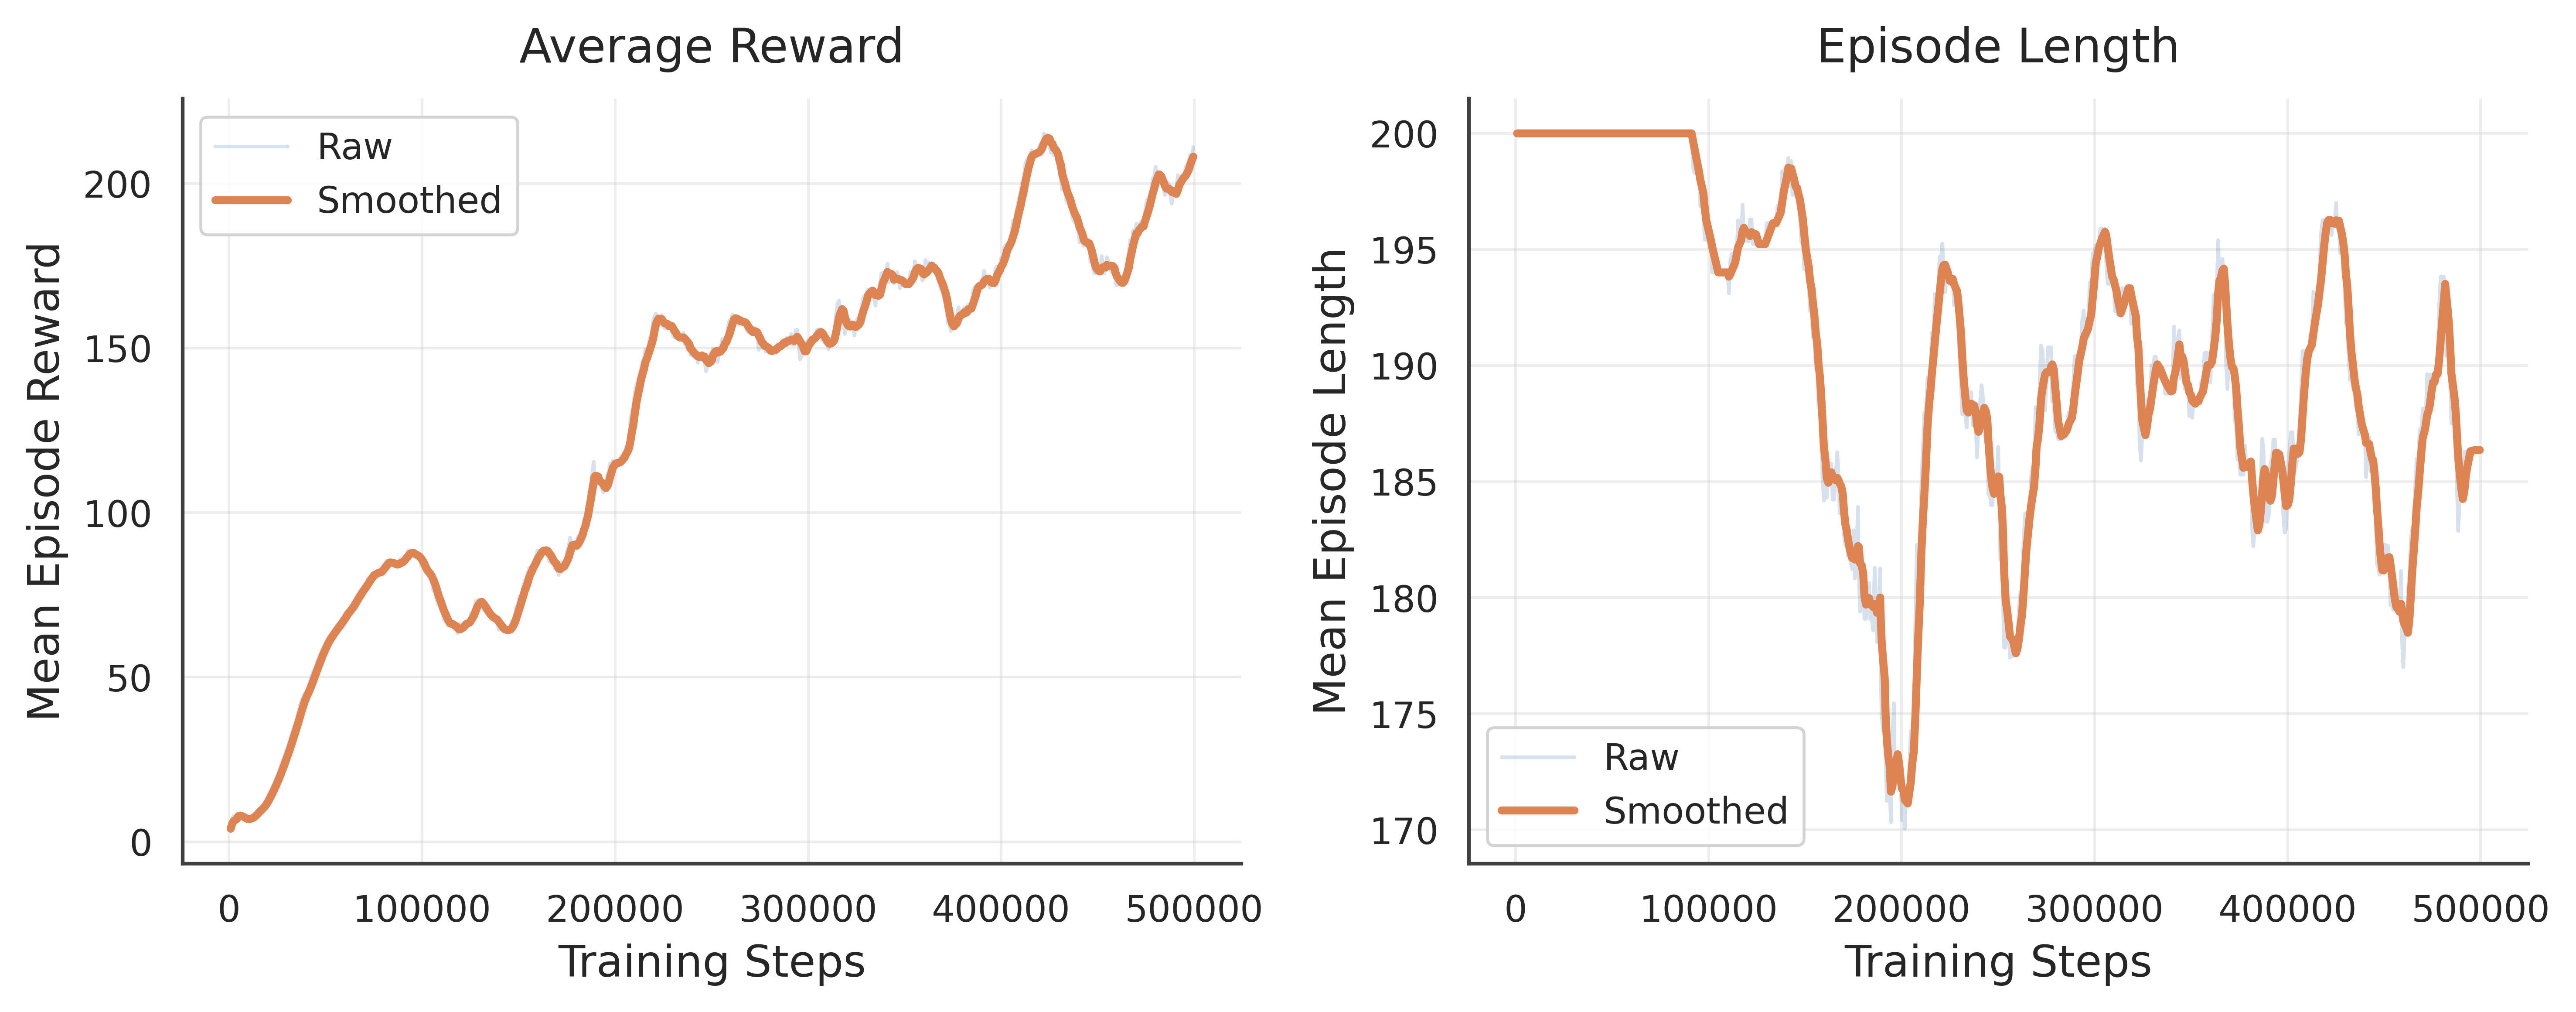
\includegraphics[width=1.0\textwidth]{fig_4_3_1_training_convergence.png}
    \caption{平均奖励与平均回合长度变化曲线}
    \label{fig:training_convergence}
  \end{figure}

由图\ref{fig:training_convergence}可以看出，在训练初期，智能体尚未掌握稳定的抓取与抬升策略，平均回合奖励处于较低水平，平均回合长度接近环境设定的最大步数。这说明随机初始化策略难以在有限时间内完成有效抓取，机械臂主要表现为探索性动作。随着训练步数增加，平均回合奖励整体呈明显上升趋势，表明智能体通过与环境持续交互，逐渐学习到接近目标物体、闭合夹爪以及抬升立方体等关键动作。

同时，平均回合长度在训练过程中整体下降，说明智能体完成任务所需的交互步数逐渐减少，策略执行效率有所提高。训练后期，平均奖励趋于较高水平并伴随一定波动，这是由于机械臂操作任务涉及接触动力学、夹爪闭合时机以及物体姿态变化等因素，强化学习训练过程本身也具有一定采样随机性。因此，奖励曲线并不会严格单调上升。综合平均回合奖励和平均回合长度的变化可以看出，SAC算法在该立方体抬升任务中能够有效提升策略性能，并逐渐形成较为稳定的操作行为。

\section{任务成功率分析}

为进一步评价 SAC 策略在立方体抬升任务中的实际完成效果，本文从任务完成程度和操作稳定性两个角度出发，设置了三类成功率指标，分别为原始抬升成功率、受控抬升成功率和稳定保持成功率。三类指标的判定标准由宽到严，能够更细致地反映智能体从“将物体抬起”到“稳定、受控地完成抬升”的策略学习过程。

其中，原始抬升成功率用于衡量立方体是否被抬升至 robosuite 环境原始成功判据所设定的高度阈值以上。该指标主要反映智能体是否具备基本的抓取与抬升能力，是最基础的任务完成指标。受控抬升成功率在原始抬升的基础上进一步引入目标高度和速度约束，即要求立方体不仅接近预设目标抬升高度，而且运动速度较小。该指标能够排除由于瞬时碰撞、快速甩动或不稳定接触导致的偶然抬升，更强调抬升过程的可控性。稳定保持成功率则要求受控抬升状态能够连续保持若干个控制步，用于评价智能体在完成抬升后是否能够维持稳定抓持与平稳保持状态，是三类指标中最严格的成功判据。

    \begin{figure}[htbp]
    \centering
    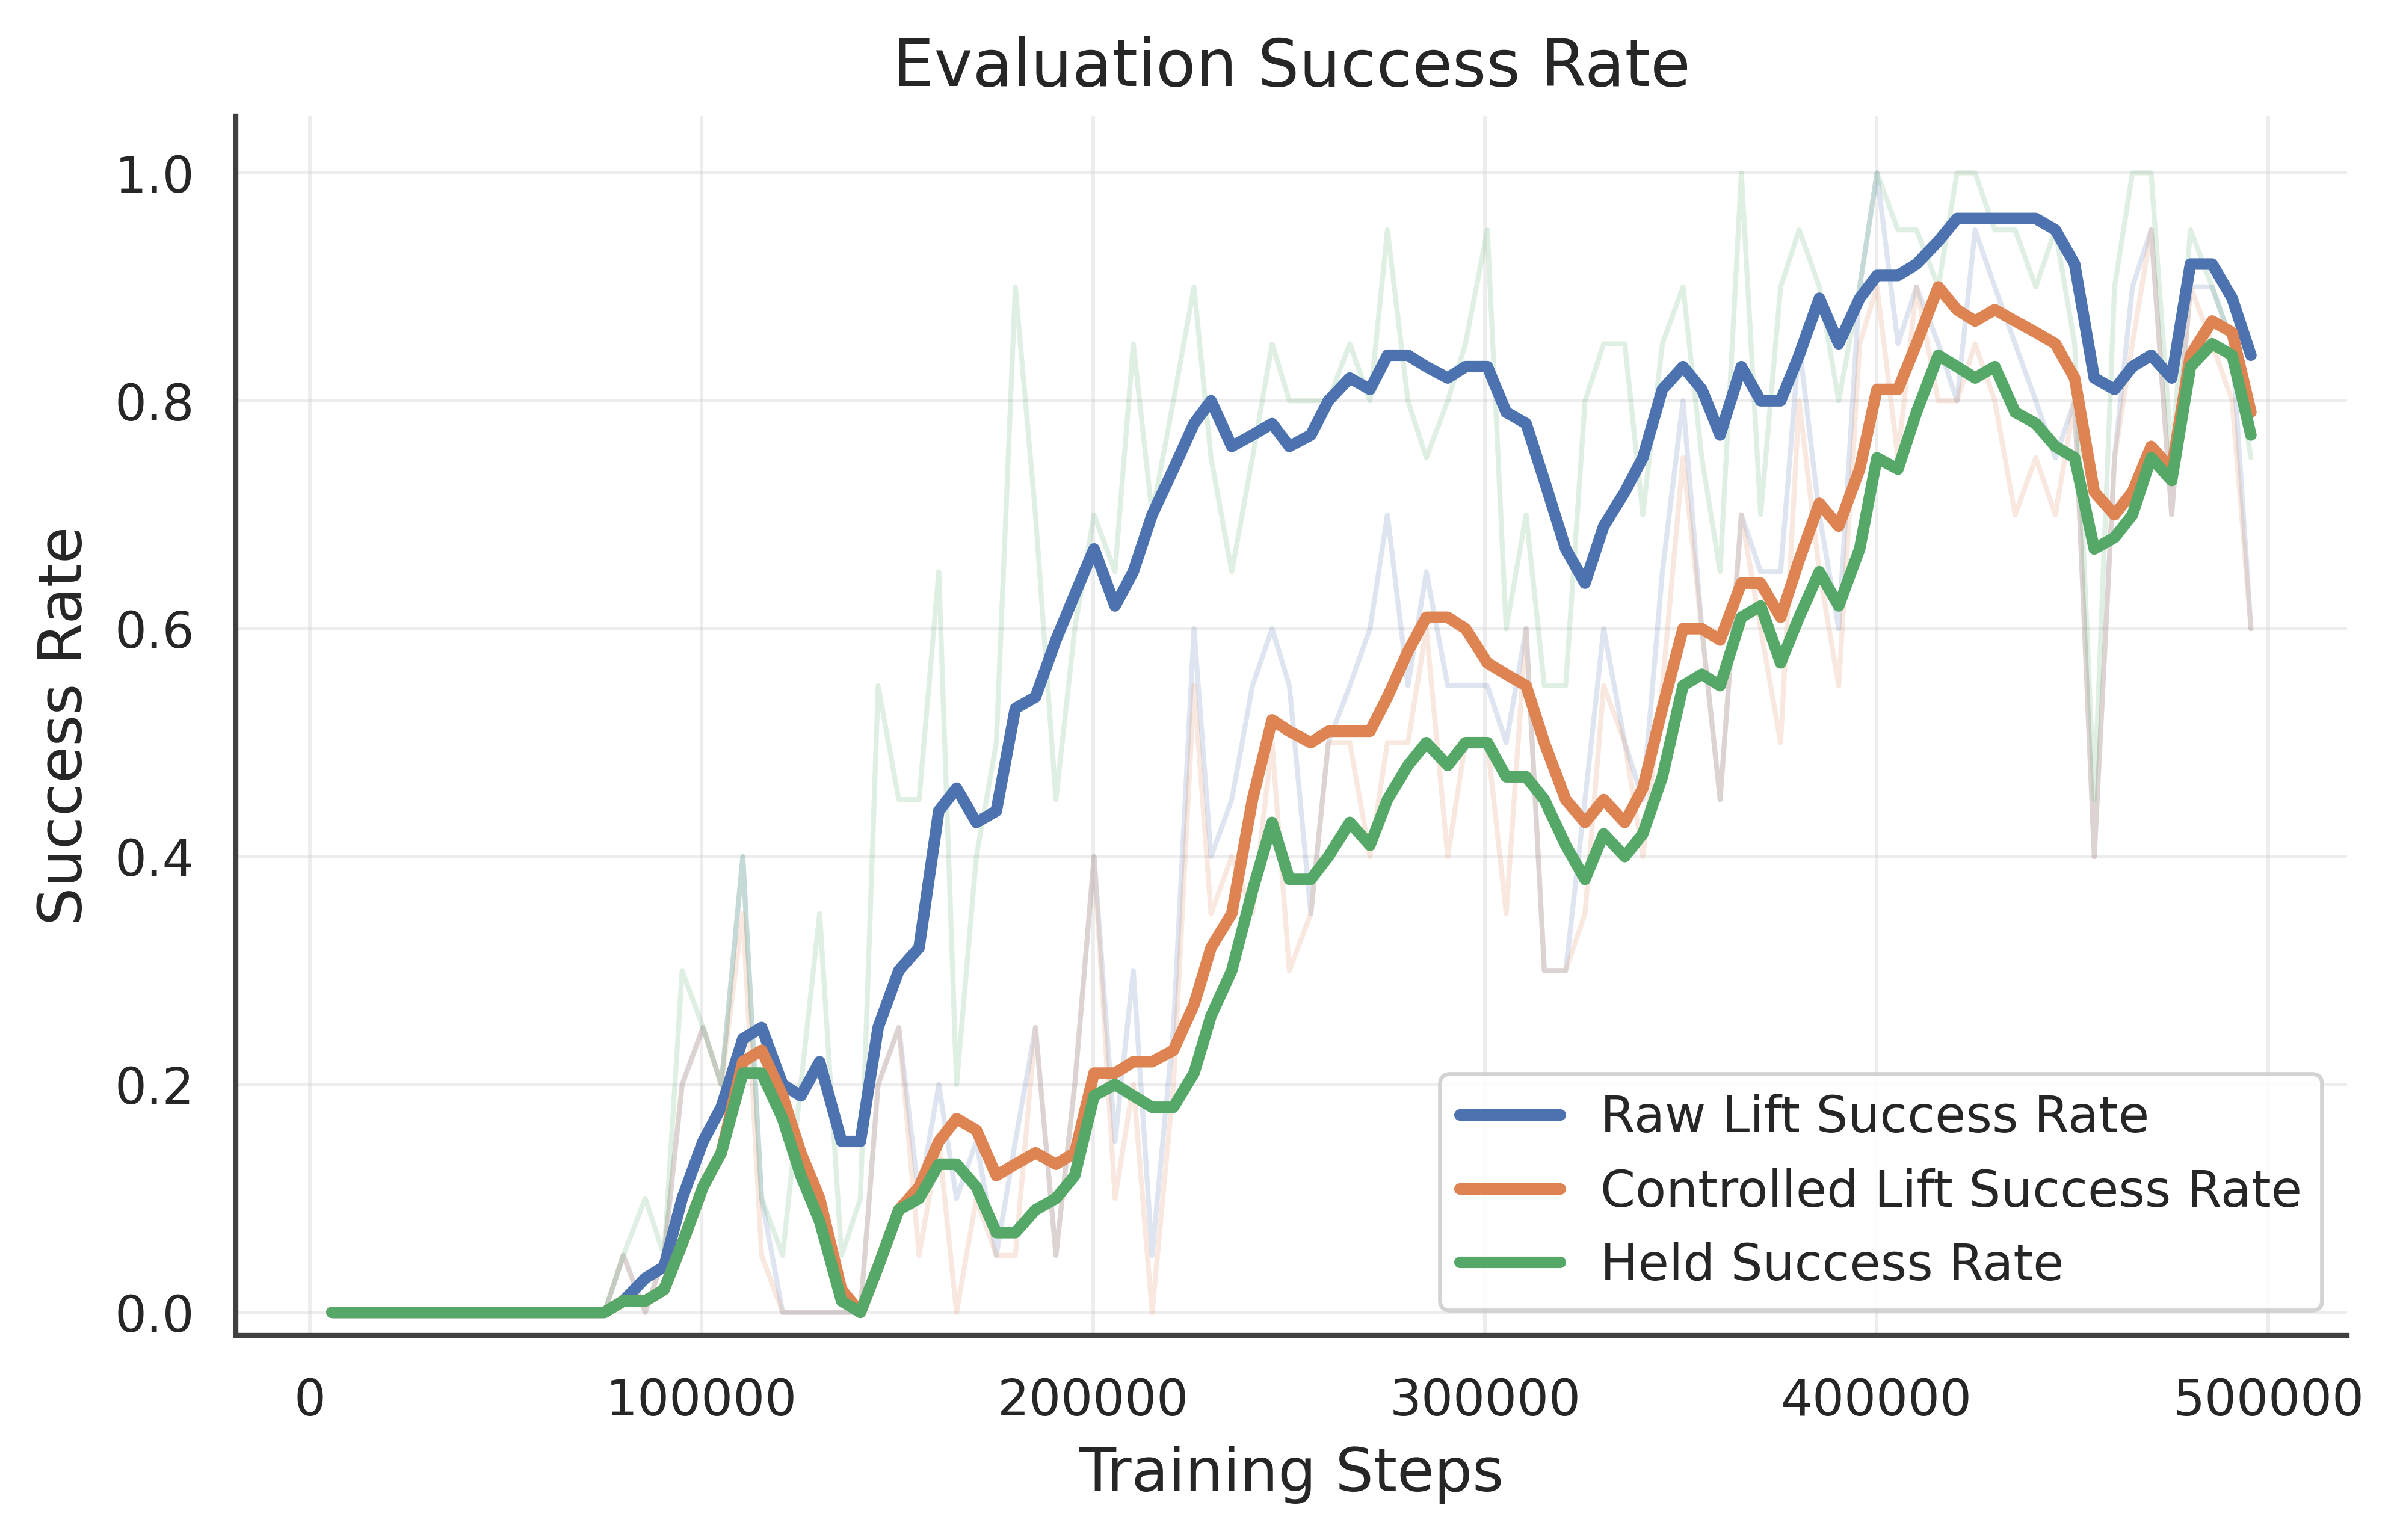
\includegraphics[width=1.0\textwidth]{fig_4_3_2_task_success_rate.png}
    \caption{评估成功率变化曲线}
    \label{fig:task_success_rate}
  \end{figure}

由图\ref{fig:task_success_rate}可以看出，在训练初期，三类成功率均接近于0，说明随机初始化策略难以完成有效的抓取与抬升操作。随着训练步数增加，三条成功率曲线整体呈上升趋势，表明 SAC 智能体在与环境持续交互的过程中，逐渐学习到了接近目标物体、闭合夹爪、抬升立方体以及保持物体稳定等关键操作行为。

从不同成功率指标的变化趋势来看，原始抬升成功率最先出现明显提升，并在训练中后期达到较高水平。这说明智能体首先学习到的是将立方体抬离桌面的基本动作策略，即能够通过夹爪接触和末端执行器上移使目标物体满足高度阈值要求。然而，原始抬升成功率较高并不意味着任务已经被稳定、受控地完成，因为该指标主要关注高度是否达到阈值，未充分约束物体运动速度和保持时间。

相比之下，受控抬升成功率的提升相对滞后，其数值整体低于原始抬升成功率。这表明在机械臂操作任务中，实现“抬起物体”相对容易，而实现“以较小速度接近目标高度并保持运动稳定”则更加困难。受控抬升成功率的持续上升说明智能体在训练后期逐渐减少了不稳定抬升、快速冲击和物体晃动等现象，策略的运动控制质量得到改善。

稳定保持成功率进一步低于原始抬升成功率，并且在训练过程中存在一定波动。这是因为稳定保持成功率不仅要求立方体达到受控抬升状态，还要求该状态连续维持若干控制步，对夹爪闭合时机、抓取姿态、末端执行器轨迹以及物体接触稳定性提出了更高要求。当夹爪与立方体之间的接触不充分，或抬升后物体出现滑移、晃动和速度过大时，稳定保持成功率就会下降。因此，该指标能够更严格地反映策略在抓取稳定性和任务鲁棒性方面的表现。

综合来看，三类成功率指标呈现出较为清晰的层次关系：原始抬升成功率最高，说明智能体已经具备基本的抬升能力；受控抬升成功率逐步提升，说明策略在目标高度控制和运动平稳性方面不断改善；稳定保持成功率在训练后期达到较高水平，说明智能体不仅能够将立方体抬起，而且能够在一定时间内维持相对稳定的受控抬升状态。该结果表明，SAC 算法能够有效学习立方体抬升任务中的关键操作策略，并逐步提升机械臂操作的成功率、可控性和稳定性。

\section{可视化行为分析}

\begin{figure}[htbp]
    \centering

    \begin{subfigure}[b]{0.45\textwidth}
        \centering
        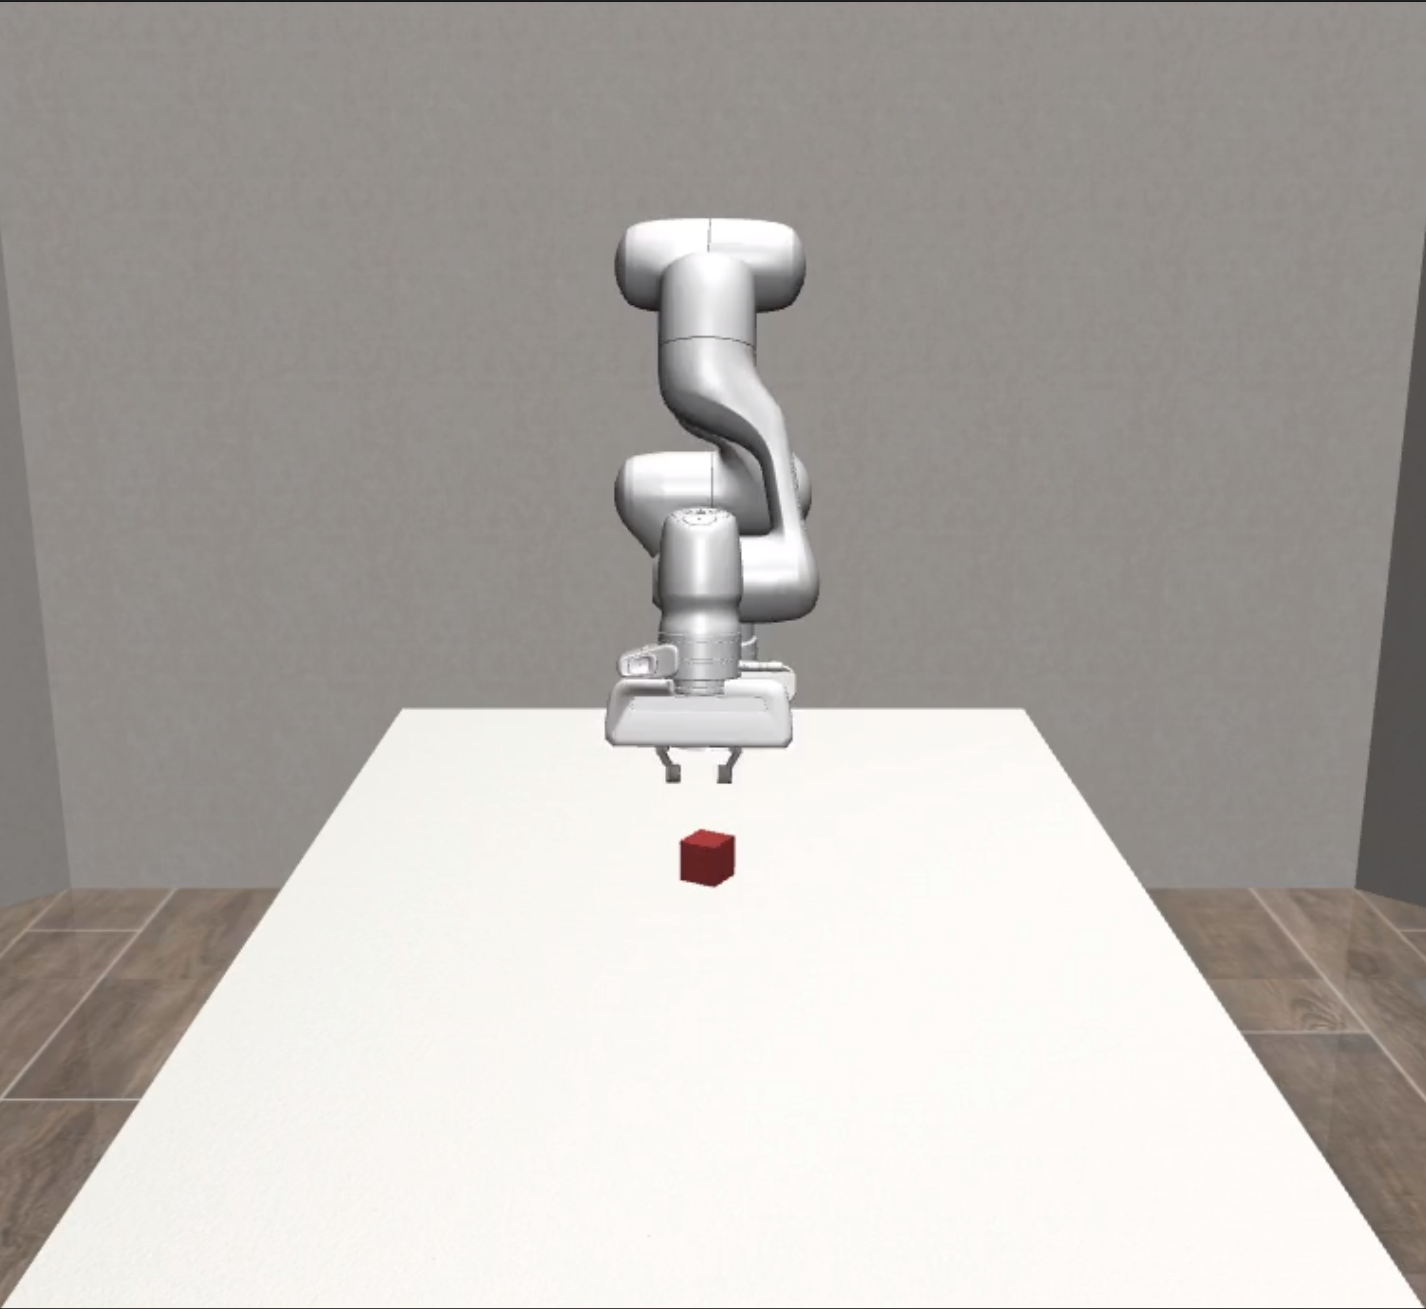
\includegraphics[width=\textwidth]{0.png}
        \caption{初始状态}
    \end{subfigure}
    \hfill
    \begin{subfigure}[b]{0.45\textwidth}
        \centering
        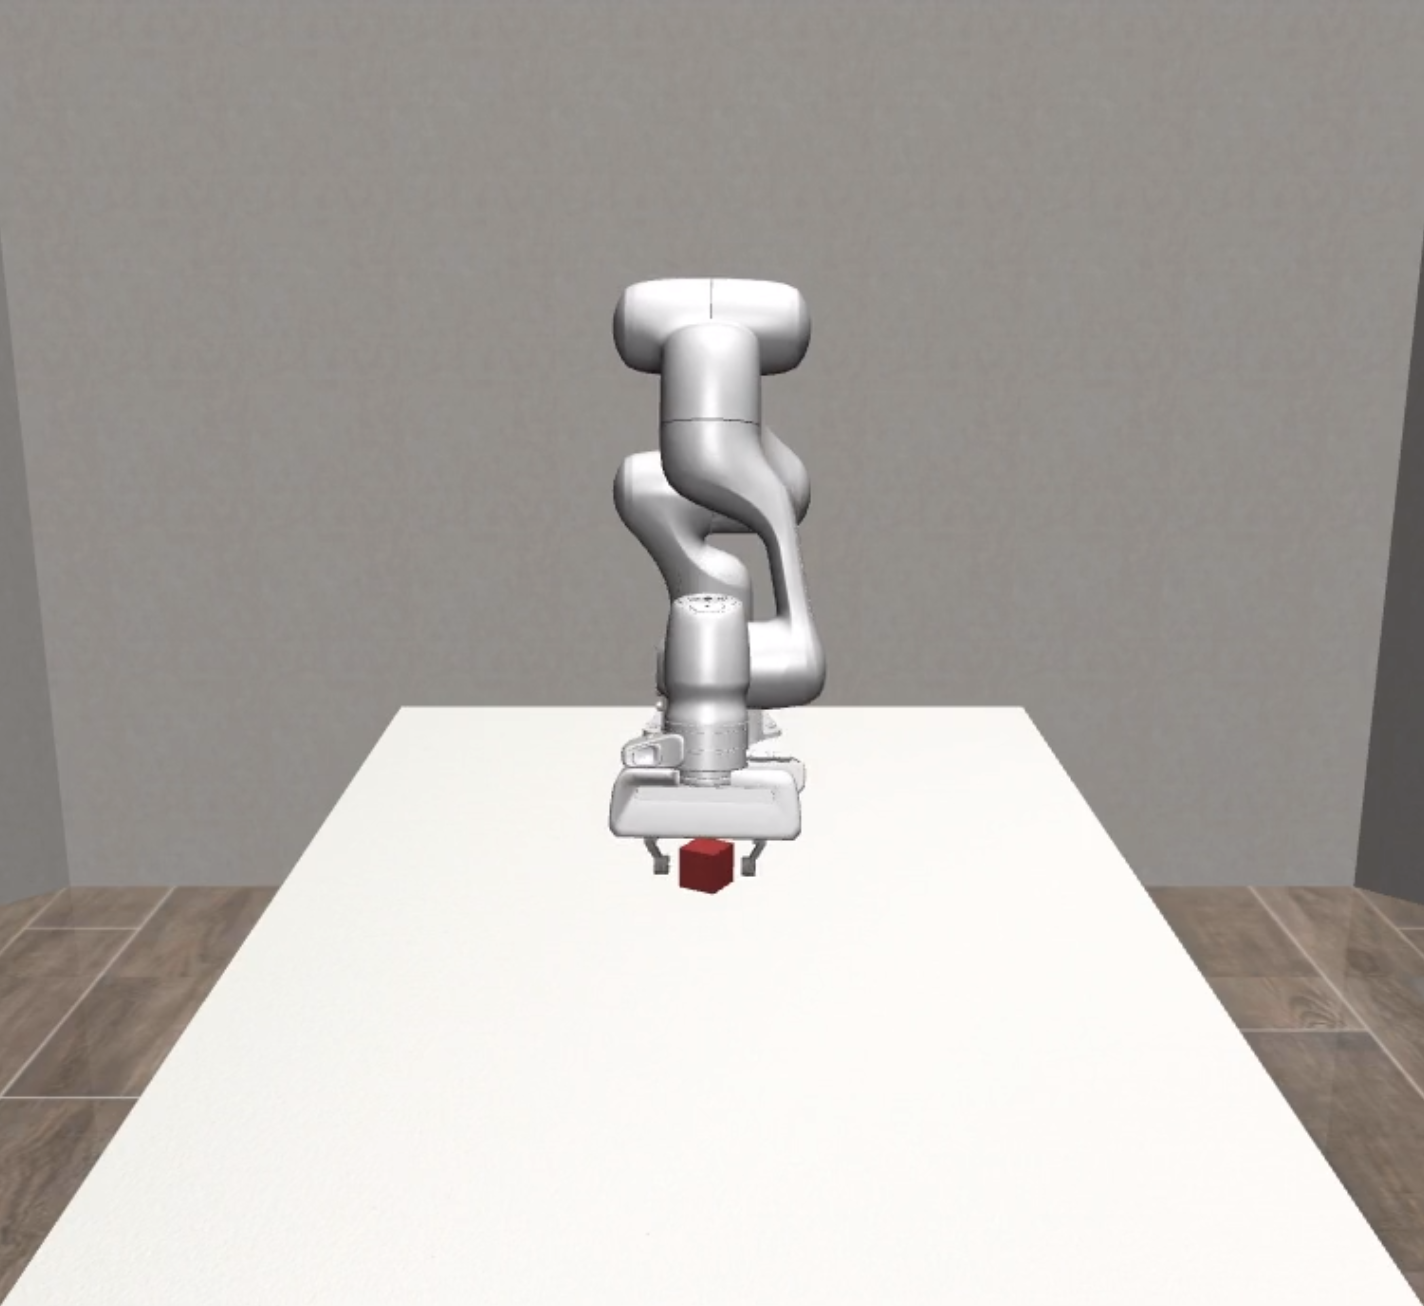
\includegraphics[width=\textwidth]{1.png}
        \caption{接近目标}
    \end{subfigure}

    \vspace{0.5em}

    \begin{subfigure}[b]{0.45\textwidth}
        \centering
        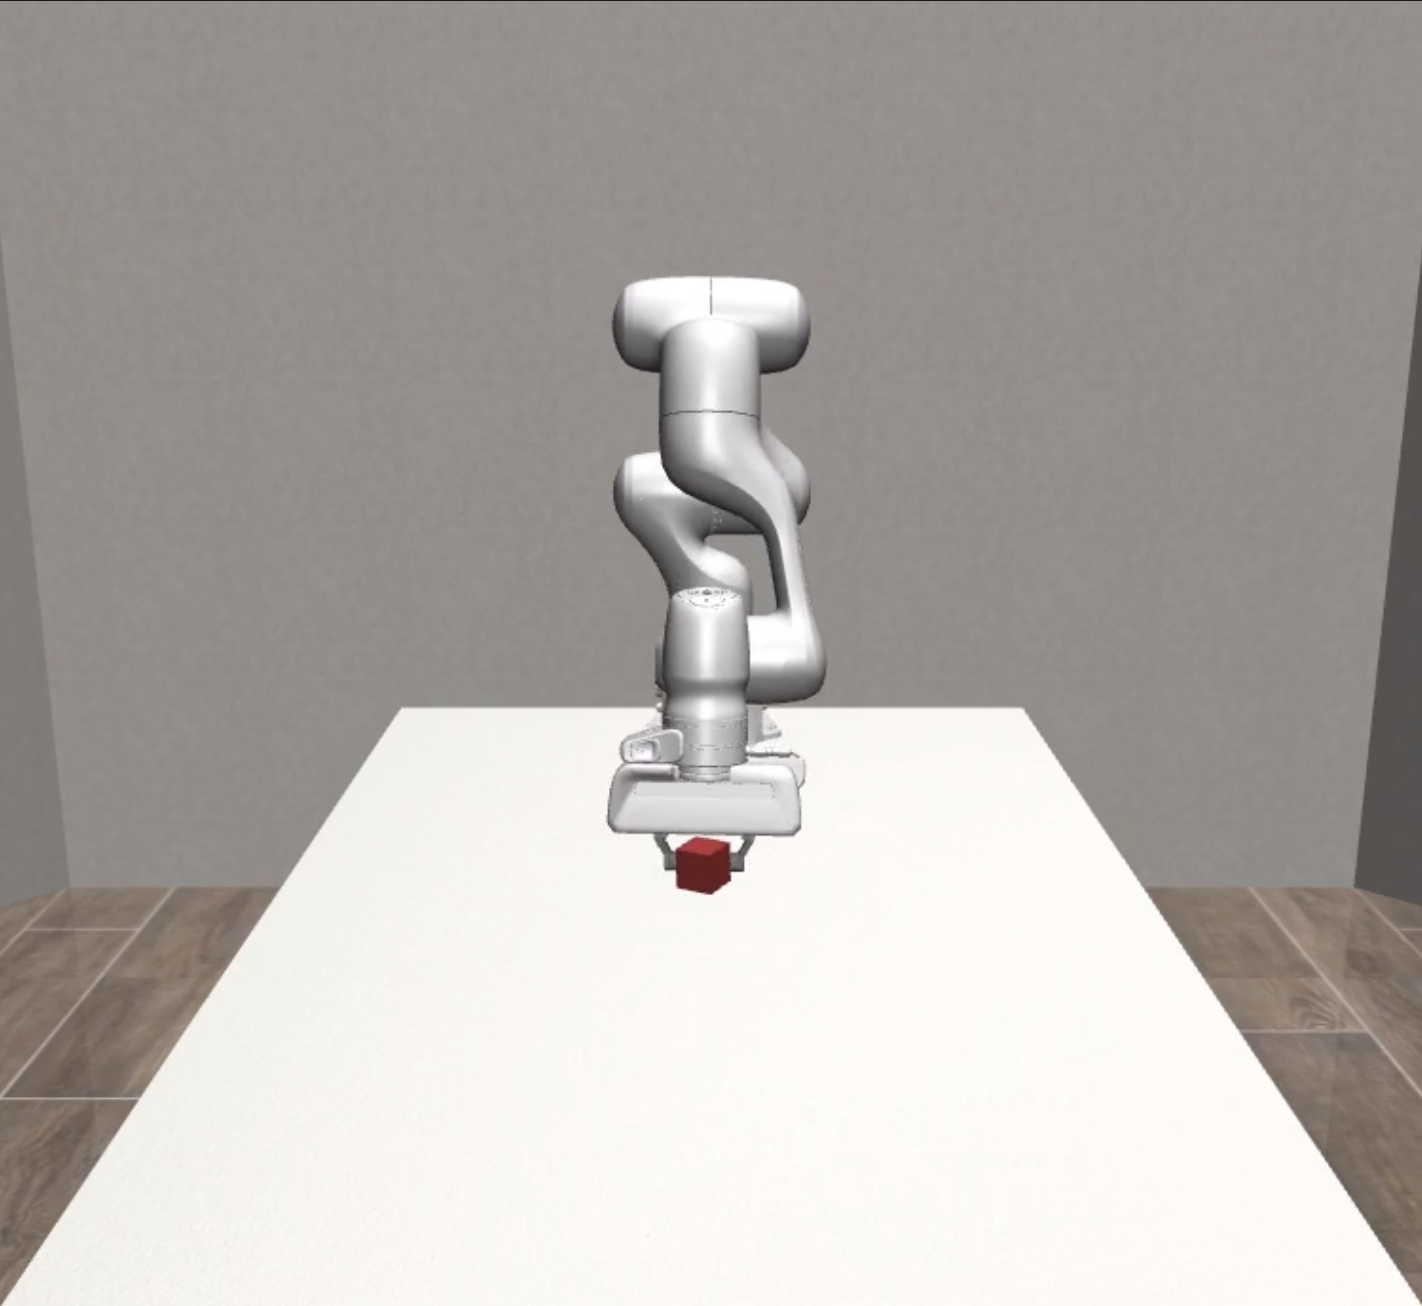
\includegraphics[width=\textwidth]{2.png}
        \caption{完成抓取}
    \end{subfigure}
    \hfill
    \begin{subfigure}[b]{0.45\textwidth}
        \centering
        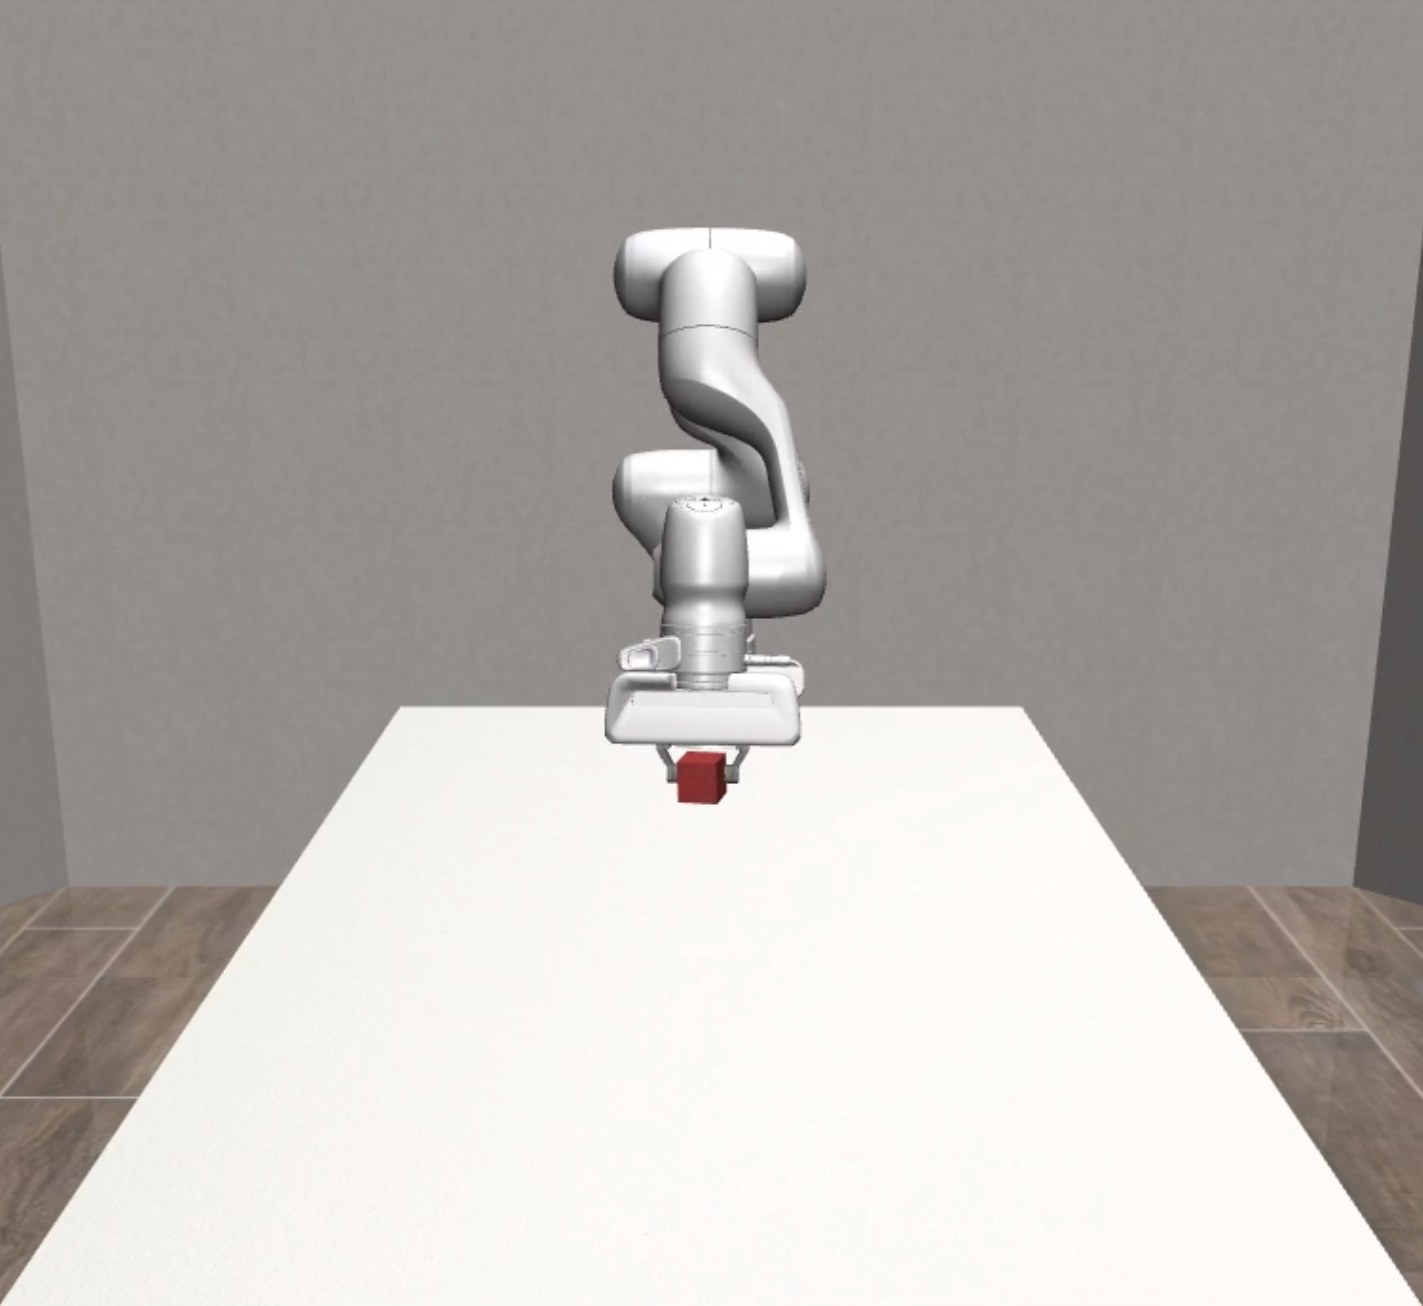
\includegraphics[width=\textwidth]{3.png}
        \caption{抬升且稳定保持}
    \end{subfigure}

    \caption{训练后SAC策略在立方体抬升任务中的可视化执行过程}
    \label{fig:sac_lift_visualization}
\end{figure}

为更加直观地展示训练后策略在立方体抬升任务中的执行效果，本文对训练完成后的 SAC 策略进行可视化测试，并选取机械臂操作过程中的若干关键帧进行展示，如图\ref{fig:sac_lift_visualization}所示。关键帧依次对应机械臂的初始状态、接近目标物体、夹爪闭合抓取、立方体抬升且稳定保持等阶段，能够较完整地反映策略执行过程中的行为变化。

可以看出，在任务开始阶段，立方体位于桌面指定区域，机械臂末端执行器处于初始位姿。随后，策略根据当前观测状态控制末端执行器逐渐向立方体靠近。在接近目标后，智能体控制夹爪闭合，实现对立方体的有效夹持。完成抓取后，机械臂末端沿竖直方向上移，将立方体抬离桌面，并最终在目标高度附近保持相对稳定。

从可视化结果可以看出，训练后的 SAC 策略能够较好地完成从“接近—抓取—抬升—保持”的连续操作过程。该过程与前文成功率曲线和抓取行为指标的变化结果相互印证：原始抬升成功率的提升说明智能体具备将物体抬离桌面的能力；受控抬升成功率的提升说明策略能够在较小速度下接近目标高度；稳定保持成功率的提升则说明智能体能够在抬升后维持较稳定的抓取状态。因此，可视化实验进一步验证了本文所训练策略在立方体抬升任务中的有效性。


\chapter{仿真到真实机械臂部署}

\section{真实系统组成}

在仿真训练完成后，本文将训练得到的最优策略部署到 Franka Research 3 真实机械臂上进行初步验证。真实系统由机械臂本体、末端夹爪、视觉感知模块、坐标变换模块、策略推理模块和安全执行模块组成。其中，机械臂平台为 Franka Research 3，末端执行器为 Franka Hand；视觉传感器采用 Intel RealSense D455 相机；物体位姿通过粘贴在立方体上的 ArUco 标记进行估计；机器人控制和坐标查询通过 ROS 2、MoveIt 2 和 TF2 完成。

真实部署流程与仿真训练流程的核心区别在于，仿真中可以直接从 MuJoCo 读取末端和物体状态，而真实系统必须通过机器人状态反馈和视觉检测获得这些量。因此，真实系统首先需要保证两个坐标链路稳定：一是机器人基坐标系到末端 TCP 坐标系的变换，二是机器人基坐标系到立方体中心坐标系的变换。只有当末端位姿和物体位姿被统一到同一个基坐标系下，仿真中训练得到的低维策略观测才可以在真实机器人上构造。

真实系统的组成如图\ref{fig:system}所示。真实系统的运行流程为首先启动 RealSense 相机节点，发布 RGB 图像和相机内参；然后启动 ArUco 检测节点，根据图像和内参估计立方体相对于相机的位姿；接着通过手眼标定外参将相机坐标系连接到机械臂基坐标系；随后启动 Franka Research 3 的 MoveIt 2 控制系统，获得末端 TCP 在基坐标系下的实时位姿；最后由真实策略执行模块加载训练得到的最优策略模型，构造真实观测、推理策略动作，并将动作转换为受限的笛卡尔线性运动。

    \begin{figure}[htbp]
    \centering
    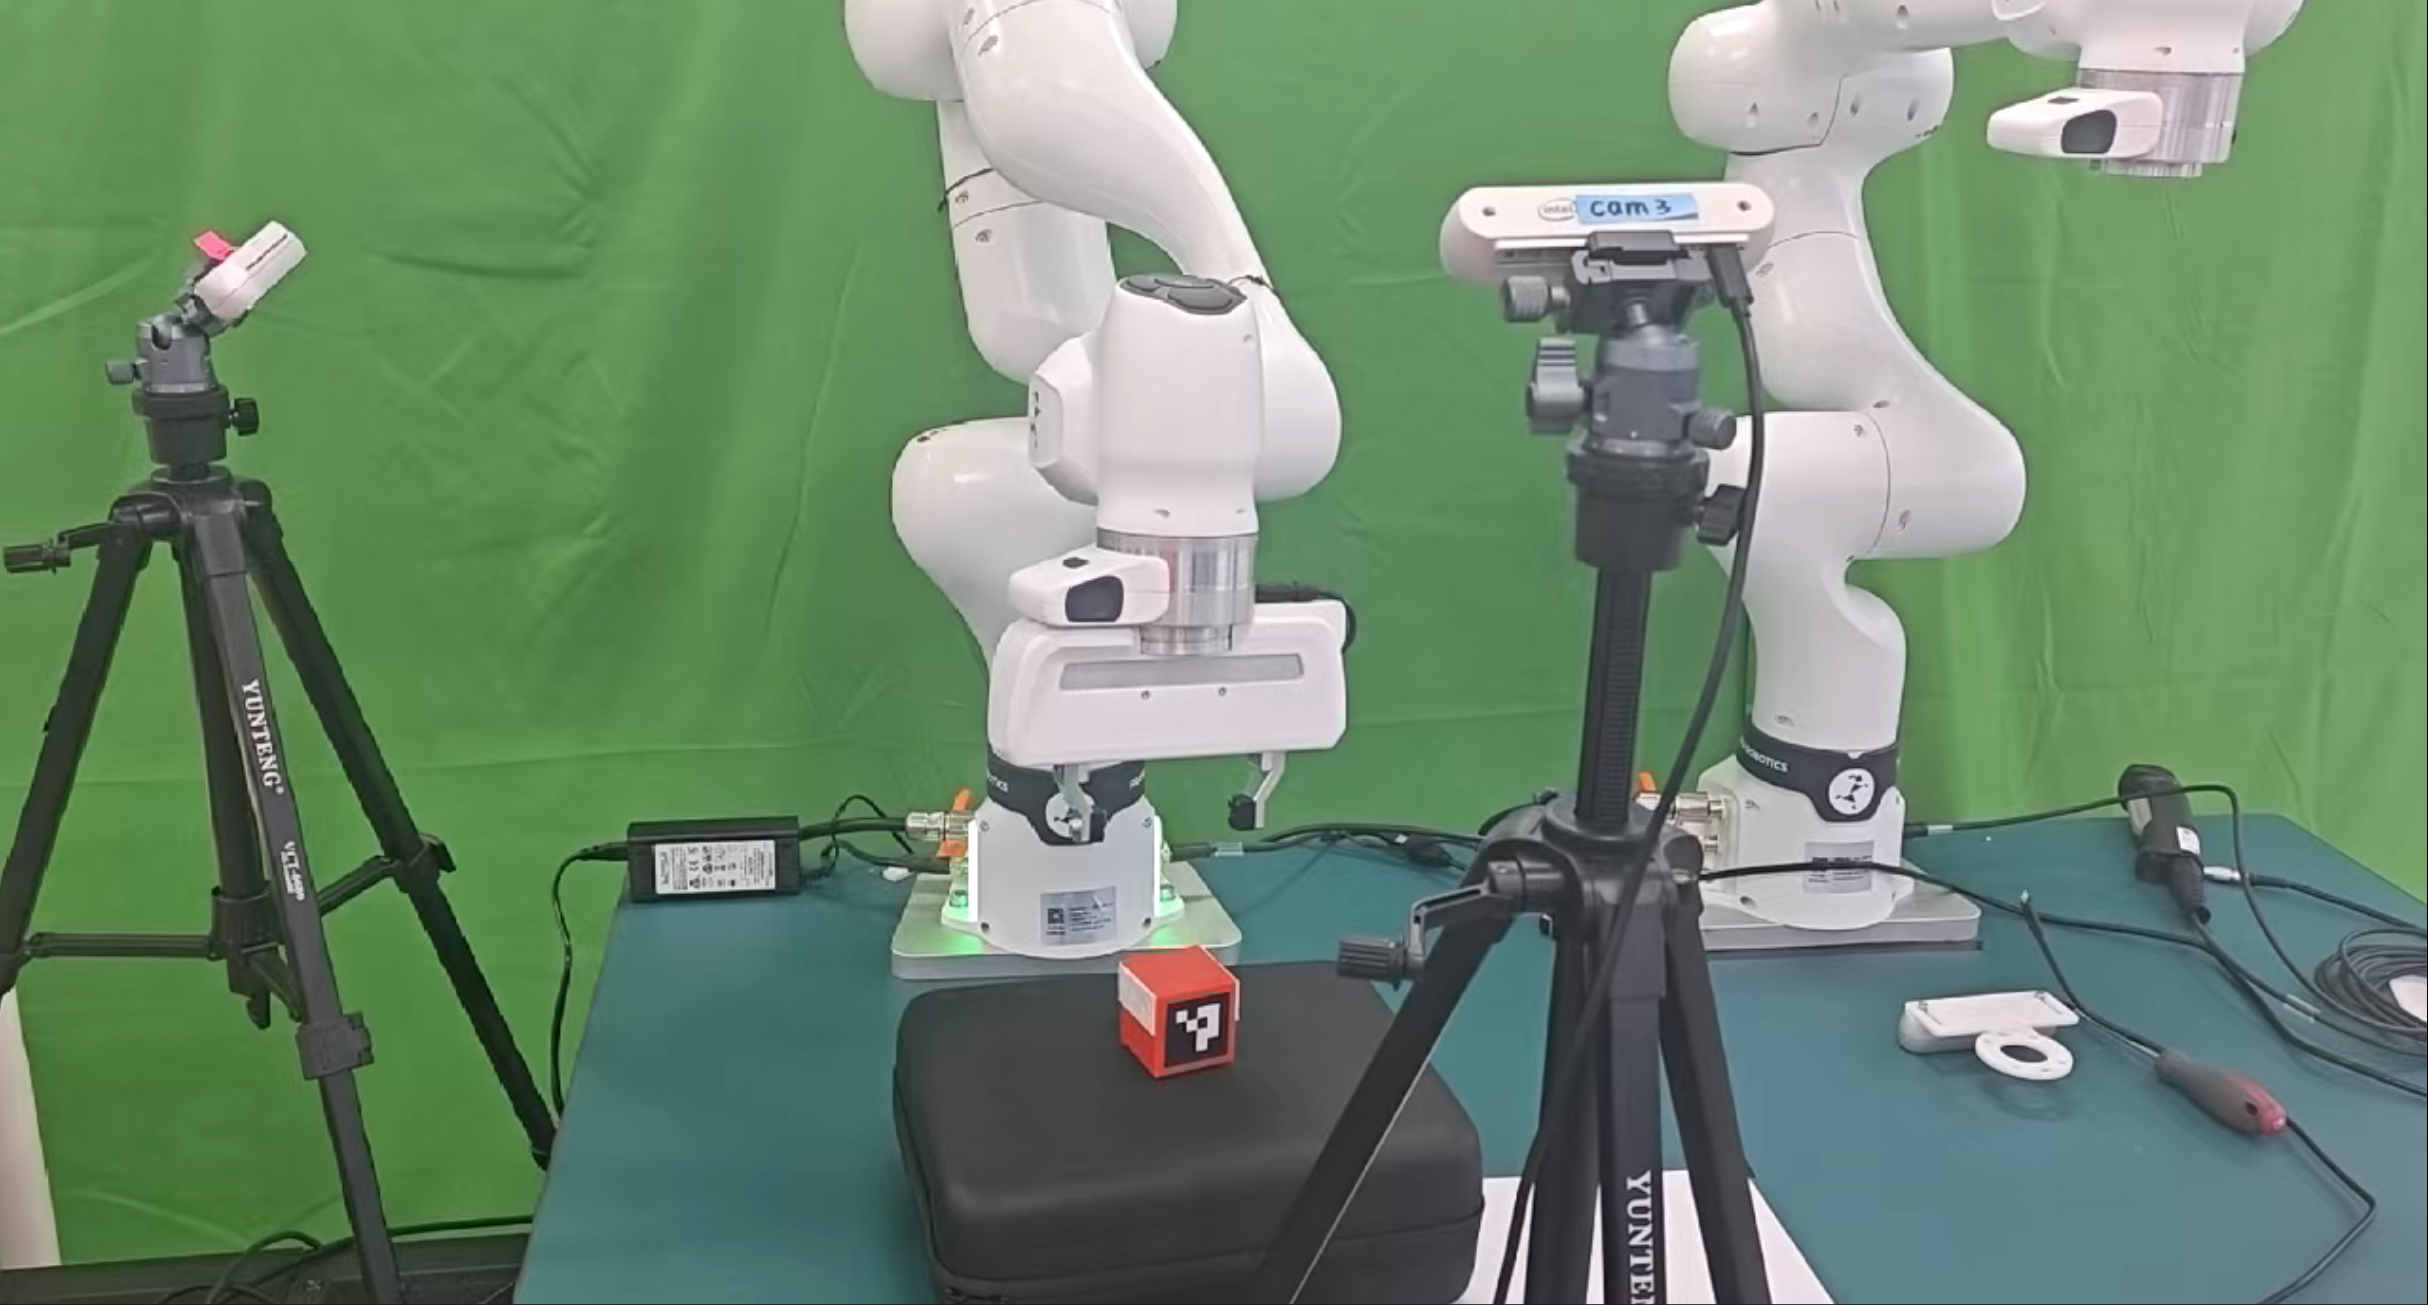
\includegraphics[width=1.0\textwidth]{4.png}
    \caption{真实系统组成}
    \label{fig:system}
  \end{figure}

% 【方法框架图占位 3：真实机器人部署总体框架图】
% 建议画出 RealSense 相机、ArUco 检测节点、手眼标定静态 TF、TF2 坐标查询、策略推理模块、MoveIt 2 笛卡尔线性控制、Franka Research 3 和 Franka Hand。
% 推荐箭头：相机图像与内参 -> ArUco 位姿估计 -> 相机坐标系下物体位姿 -> 机器人基坐标系下物体位姿；物体位姿与末端位姿 -> 观测向量 -> SAC 策略 -> 动作缩放与夹爪控制 -> MoveIt/夹爪控制 -> 机器人执行。

\section{视觉定位与坐标变换}

RealSense D455 相机以 RGB 模式运行，图像分辨率设置为 $1280\times720$，帧率为 30 Hz。相机节点发布彩色图像和相机内参。ArUco 检测节点订阅上述图像和内参，识别贴在立方体上的标记，并发布立方体在相机光学坐标系下的位姿。该位姿进一步作为 TF 中的物体坐标系。

本文只使用 RGB 图像进行 ArUco 位姿估计，因此关闭深度流。这样可以减少系统带宽和节点计算负担，同时避免深度噪声对位姿估计产生额外影响。相机内参信息包含相机内参矩阵、畸变参数和图像分辨率。ArUco 节点根据内参将标记角点从像素坐标反投影到三维空间，并结合标记实际边长估计标记相对于相机的 6D 位姿。

在实现中，视觉定位模块订阅彩色图像和相机内参，并输出立方体在相机标定光学坐标系下的位置和姿态。该输出包含立方体中心位置 $p$ 和姿态四元数 $q$。节点同时将检测到的立方体位姿发布为 TF 中的物体坐标系，使后续控制程序可以直接通过 TF2 查询机器人基坐标系到立方体的变换。由于本文策略主要依赖末端位置、物体位置和相对位置完成抓取，物体姿态主要用于保持与仿真观测维度一致。

为了将相机检测结果转换到机器人基坐标系，本文使用手眼标定得到机器人基坐标系到相机标定光学坐标系的外参。实机实验中使用的平移向量为
\begin{equation}
  \boldsymbol{t}_{base}^{camera} =
  [0.7075,\ 0.1160,\ 0.5924]^T \ \mathrm{m},
\end{equation}
对应四元数为
\begin{equation}
  \boldsymbol{q}_{base}^{camera} =
  [-0.6614,\ -0.6717,\ 0.2179,\ 0.2526].
\end{equation}
通过 ROS 2 静态 TF 发布该外参后，系统可以查询完整的坐标链：
\begin{equation}
  \mathrm{base} \rightarrow
  \mathrm{camera} \rightarrow
  \mathrm{cube}.
\end{equation}

手眼标定的作用可以用齐次变换表示。设 ${}^{base}T_{camera}$ 为相机坐标系到机器人基坐标系的变换，${}^{camera}T_{cube}$ 为 ArUco 检测得到的立方体相对于相机的变换，则立方体在机器人基坐标系下的位姿为
\begin{equation}
  {}^{base}T_{cube}
  =
  {}^{base}T_{camera}
  {}^{camera}T_{cube}.
\end{equation}
该公式说明，真实部署中所有用于策略推理的位置量必须先统一到机器人基坐标系。若直接将相机坐标系下的物体位置输入策略，坐标轴方向、原点位置和尺度含义都会与仿真训练不一致，策略输出将失去物理意义。

本文将手眼标定结果作为静态坐标变换发布到 TF 系统中。发布该静态变换后，可以分别检查机器人基坐标系到立方体坐标系、机器人基坐标系到末端 TCP 坐标系的变换结果。前者用于检查物体是否位于真实桌面任务区域，后者用于检查机械臂 TCP 位姿是否正常。只有这两个查询都稳定输出，才说明真实策略推理所需的坐标链已经建立。

实机测试中，TF 查询能够得到稳定的立方体位置。例如某次测试中，立方体在机器人基坐标系下的位置约为
\begin{equation}
  \boldsymbol{p}_{cube}^{base}=[0.436,\ 0.056,\ 0.130]^T \ \mathrm{m},
\end{equation}
末端 TCP 位姿查询结果约为
\begin{equation}
  \boldsymbol{p}_{eef}^{base}=[0.410,\ -0.034,\ 0.286]^T \ \mathrm{m}.
\end{equation}
这说明视觉定位结果已经被转换到了与机器人末端一致的坐标系中，可以用于真实策略推理。

% 【方法框架图占位 4：真实系统坐标变换框架图】
% 建议画出机器人基坐标系、相机坐标系、物体坐标系、末端 TCP 坐标系，以及手眼标定外参、视觉检测外参和最终位姿查询关系。
% 可在图中标明物体位置、末端位置和相对位置均在机器人基坐标系下计算。

\section{真实观测构造}

本文在真实机器人上保持与仿真训练一致的低维观测结构。真实观测向量为
\begin{equation}
  \boldsymbol{o} =
  [\boldsymbol{p}_{eef},\ g,\ \boldsymbol{p}_{cube},\
  \boldsymbol{q}_{cube},\ \boldsymbol{p}_{cube}-\boldsymbol{p}_{eef}],
\end{equation}
其中所有位置量均在机器人基坐标系下表示，$g$ 表示夹爪开合状态，$\boldsymbol{q}_{cube}$ 表示立方体姿态四元数。该观测结构与仿真中的 14 维低维状态保持一致，从而避免在真实部署时改变策略网络输入维度。

需要注意的是，真实系统中的物体位姿来自视觉检测，因此会受到标记检测误差、相机噪声和时间延迟影响。为了降低噪声对动作的影响，真实执行程序对策略输出的位置动作进行了低通滤波，并设置了每步最大末端位移限制。这样可以在保持策略趋势的同时，避免单帧视觉抖动导致机械臂产生突然运动。

真实观测由策略执行模块完成。该模块首先读取控制器维护的当前 TCP 位姿，然后通过 TF2 查询机器人基坐标系到立方体坐标系的变换，最后计算相对位置
\begin{equation}
  \boldsymbol{p}_{rel}
  =
  \boldsymbol{p}_{cube}^{base}
  -
  \boldsymbol{p}_{eef}^{base}.
\end{equation}
程序将末端位置、夹爪开合状态、立方体位置、立方体四元数和相对位置按训练时相同顺序拼接为 NumPy 数组，并输入到 SAC 策略网络中。这样做的关键是保持真实观测和仿真观测在维度、顺序、单位和坐标系上的一致性。

在程序启动阶段，系统会持续检查两个条件：第一，控制器已经能够提供末端 TCP 位姿；第二，TF2 能够查询机器人基坐标系到立方体坐标系的变换。如果相机没有看到 ArUco 标记，或者静态手眼标定 TF 没有发布，系统会等待而不会进入执行阶段。这一设计可以避免在观测不完整时向真实机械臂发送错误动作。

\section{动作执行与安全裁剪}

训练策略输出的动作为
\begin{equation}
  \boldsymbol{a}=[a_x,\ a_y,\ a_z,\ a_g]^T,
\end{equation}
其中前三维为归一化的末端位置增量，第四维为夹爪开合动作。真实部署时不能将 $a_x,a_y,a_z$ 直接作为米制位移，而是先按照仿真中操作空间位置控制器的动作尺度转换为末端位移。本文实机实验中以 0.05 m 作为归一化动作的基础尺度，并将单次真实执行位移限制在 1 mm 左右。实际执行命令可表示为
\begin{equation}
  \Delta \boldsymbol{x}_{real}
  = \mathrm{clip}(\alpha \boldsymbol{a}_{xyz}, -\Delta_{max}, \Delta_{max}),
\end{equation}
其中 $\alpha$ 为动作尺度系数，$\Delta_{max}$ 为真实机器人单步位移上限。

真实机械臂的笛卡尔运动通过 MoveIt 2 的笛卡尔线性路径接口执行。控制模块将每一步策略输出转换为一个小幅度 TCP 目标位置，再由 MoveIt 2 规划并执行线性笛卡尔路径。相比直接使用普通位姿规划，这种方式更接近仿真中的操作空间位置增量控制形式，也更适合低速、安全地验证强化学习策略。

夹爪动作由策略输出的第四维 $a_g$ 决定。当 $a_g$ 小于设定阈值时，真实系统触发 Franka Hand 闭合命令；闭合完成后，程序执行一个小幅度竖直抬升动作，用于验证物体是否被成功抓取并离开桌面。实机实验中使用的抬升高度为 0.075 m，与第一阶段仿真训练目标一致。

真实策略执行模块在每个控制周期中首先构造真实观测，然后加载策略模型进行确定性推理，得到四维动作。随后，动作转换模块将前三维动作转换为真实末端位移。该过程包含三层安全处理：第一，对策略动作裁剪到 $[-1,1]$；第二，对动作做低通滤波，避免视觉噪声导致动作跳变；第三，将位移裁剪到预设的最大单步距离，并进一步限制到设定工作空间内。

真实执行阶段还设置了较低的策略执行频率、较小的单步末端位移、未抓取前的最低接近高度、夹爪使能开关以及抓取后的竖直抬升动作。线性运动控制模块负责将目标末端位置发送给 MoveIt 2，由笛卡尔路径接口生成线性 TCP 轨迹。相较于普通位姿规划，笛卡尔线性路径更容易保持末端运动方向与策略输出一致，能够减少绕行和姿态突变。夹爪闭合由策略第四维动作 $a_g$ 触发，当该动作小于阈值时，系统执行 Franka Hand 闭合。


\section{真实机械臂验证结果}

完成相机标定、TF 坐标链配置和控制程序调试后，本文在 Franka Research 3 真实机械臂上进行了 sim-to-real 初步验证。实验过程中，RealSense 相机持续检测立方体位姿，TF 系统实时提供机器人基坐标系下的立方体位姿和末端位姿。策略执行模块加载仿真训练得到的最优策略模型，按照 1 Hz 左右的低频率输出动作，并通过笛卡尔线性控制接口执行。

\begin{figure}[htbp]
    \centering

    \begin{subfigure}[b]{0.45\textwidth}
        \centering
        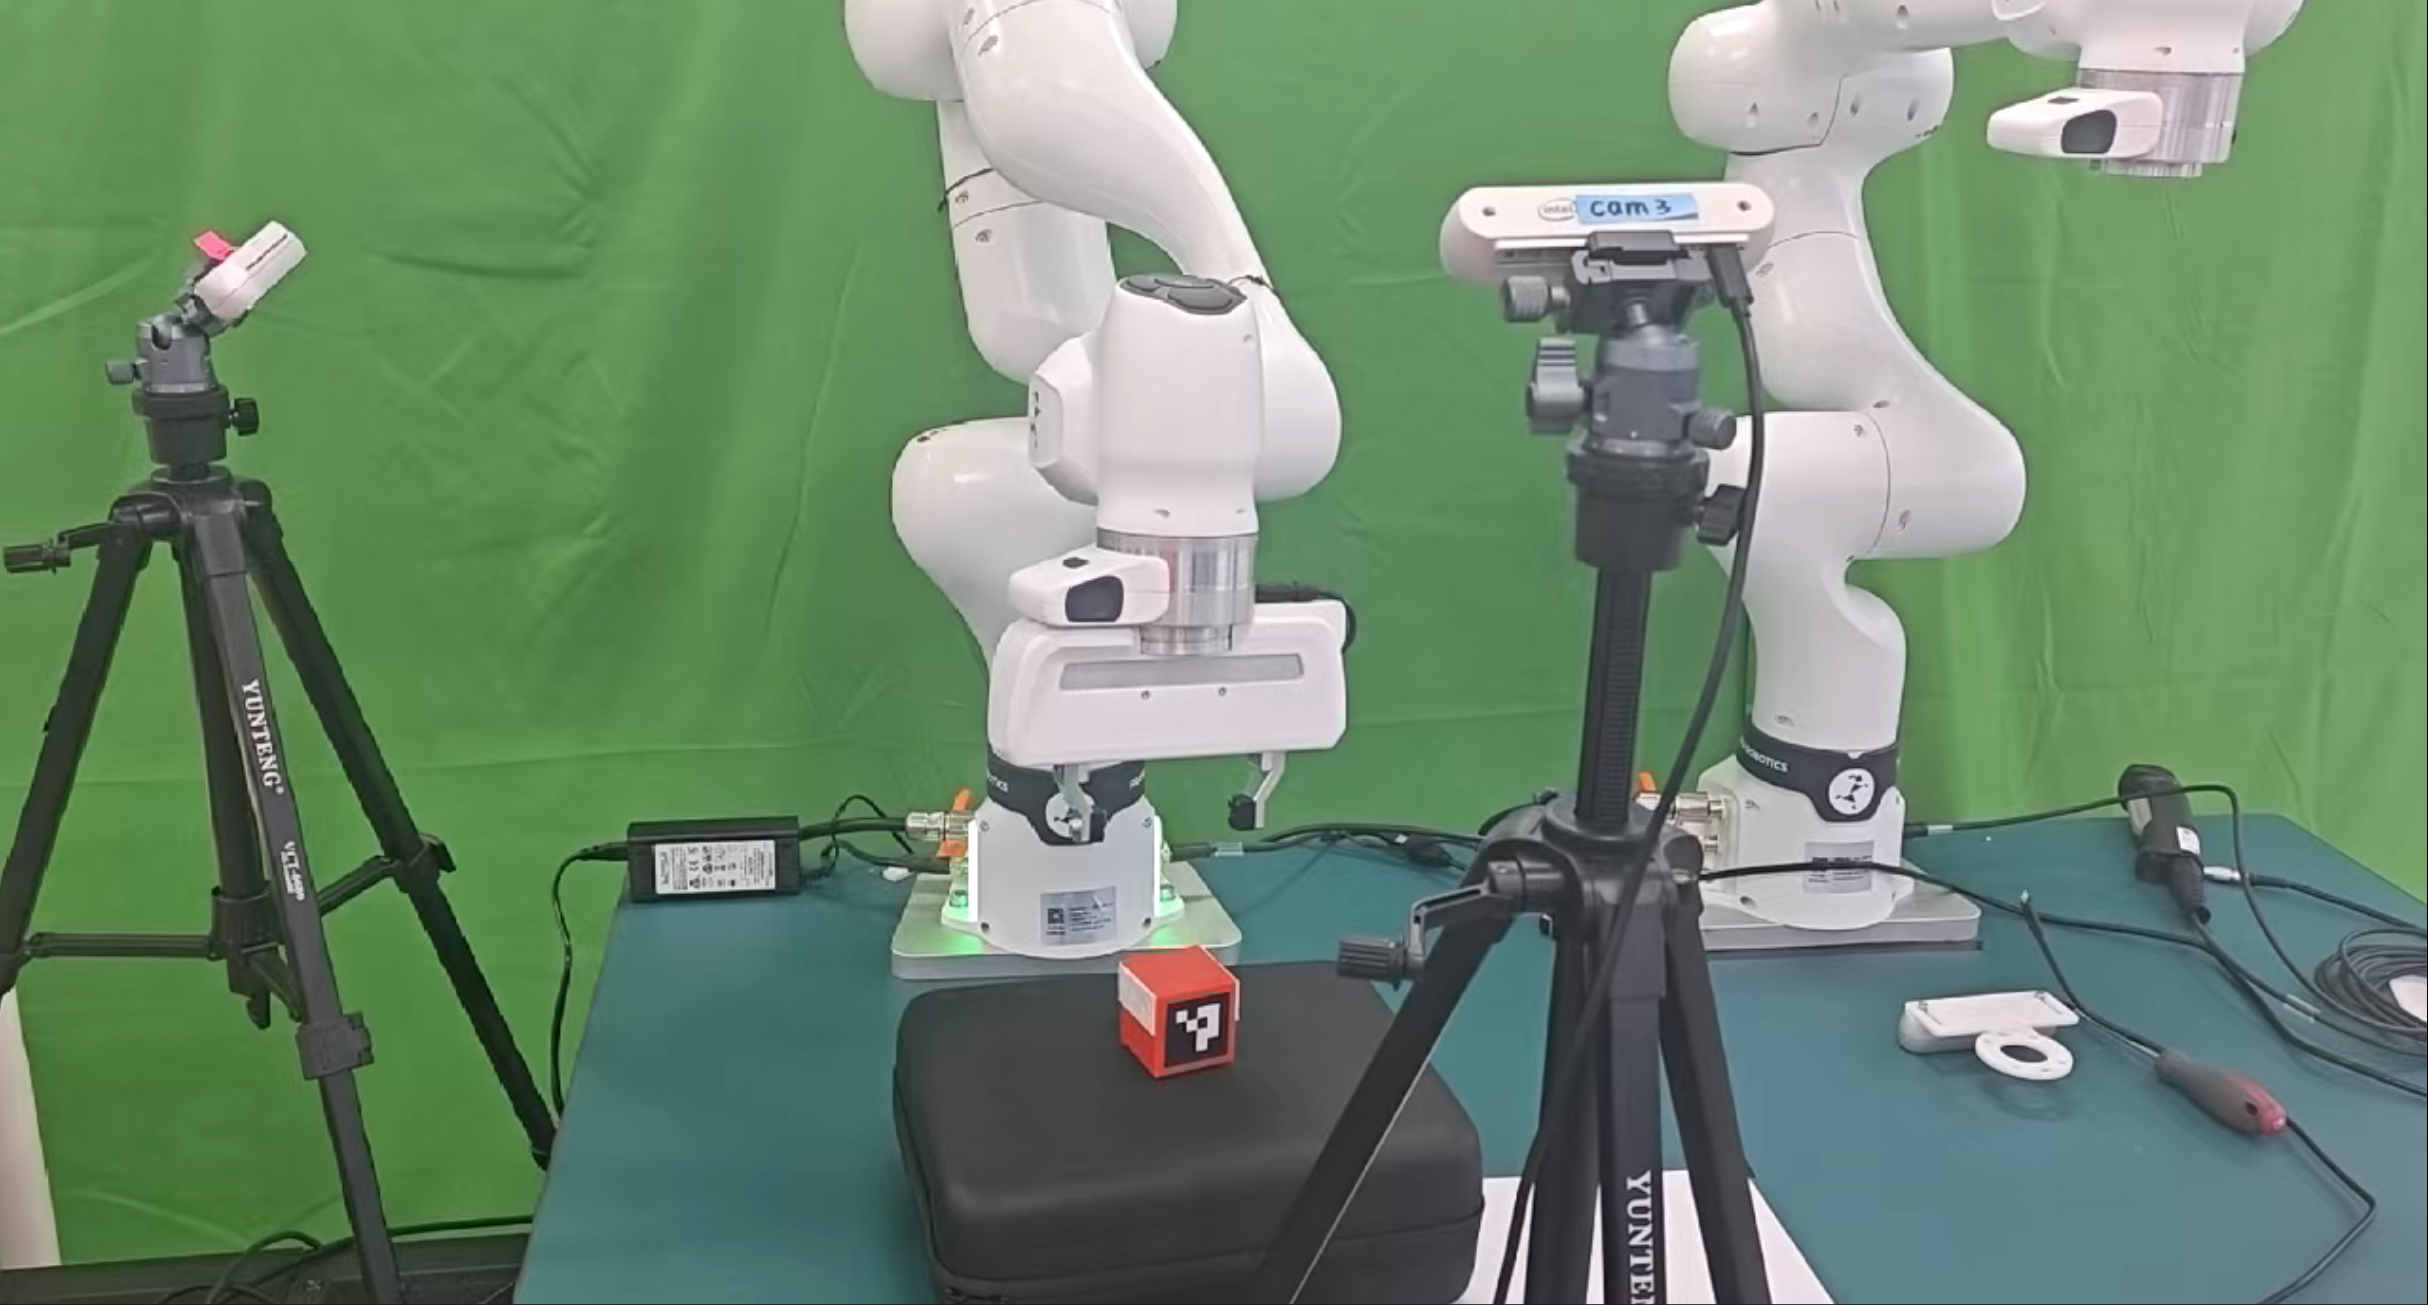
\includegraphics[width=\textwidth]{4.png}
        \caption{初始状态}
    \end{subfigure}
    \hfill
    \begin{subfigure}[b]{0.45\textwidth}
        \centering
        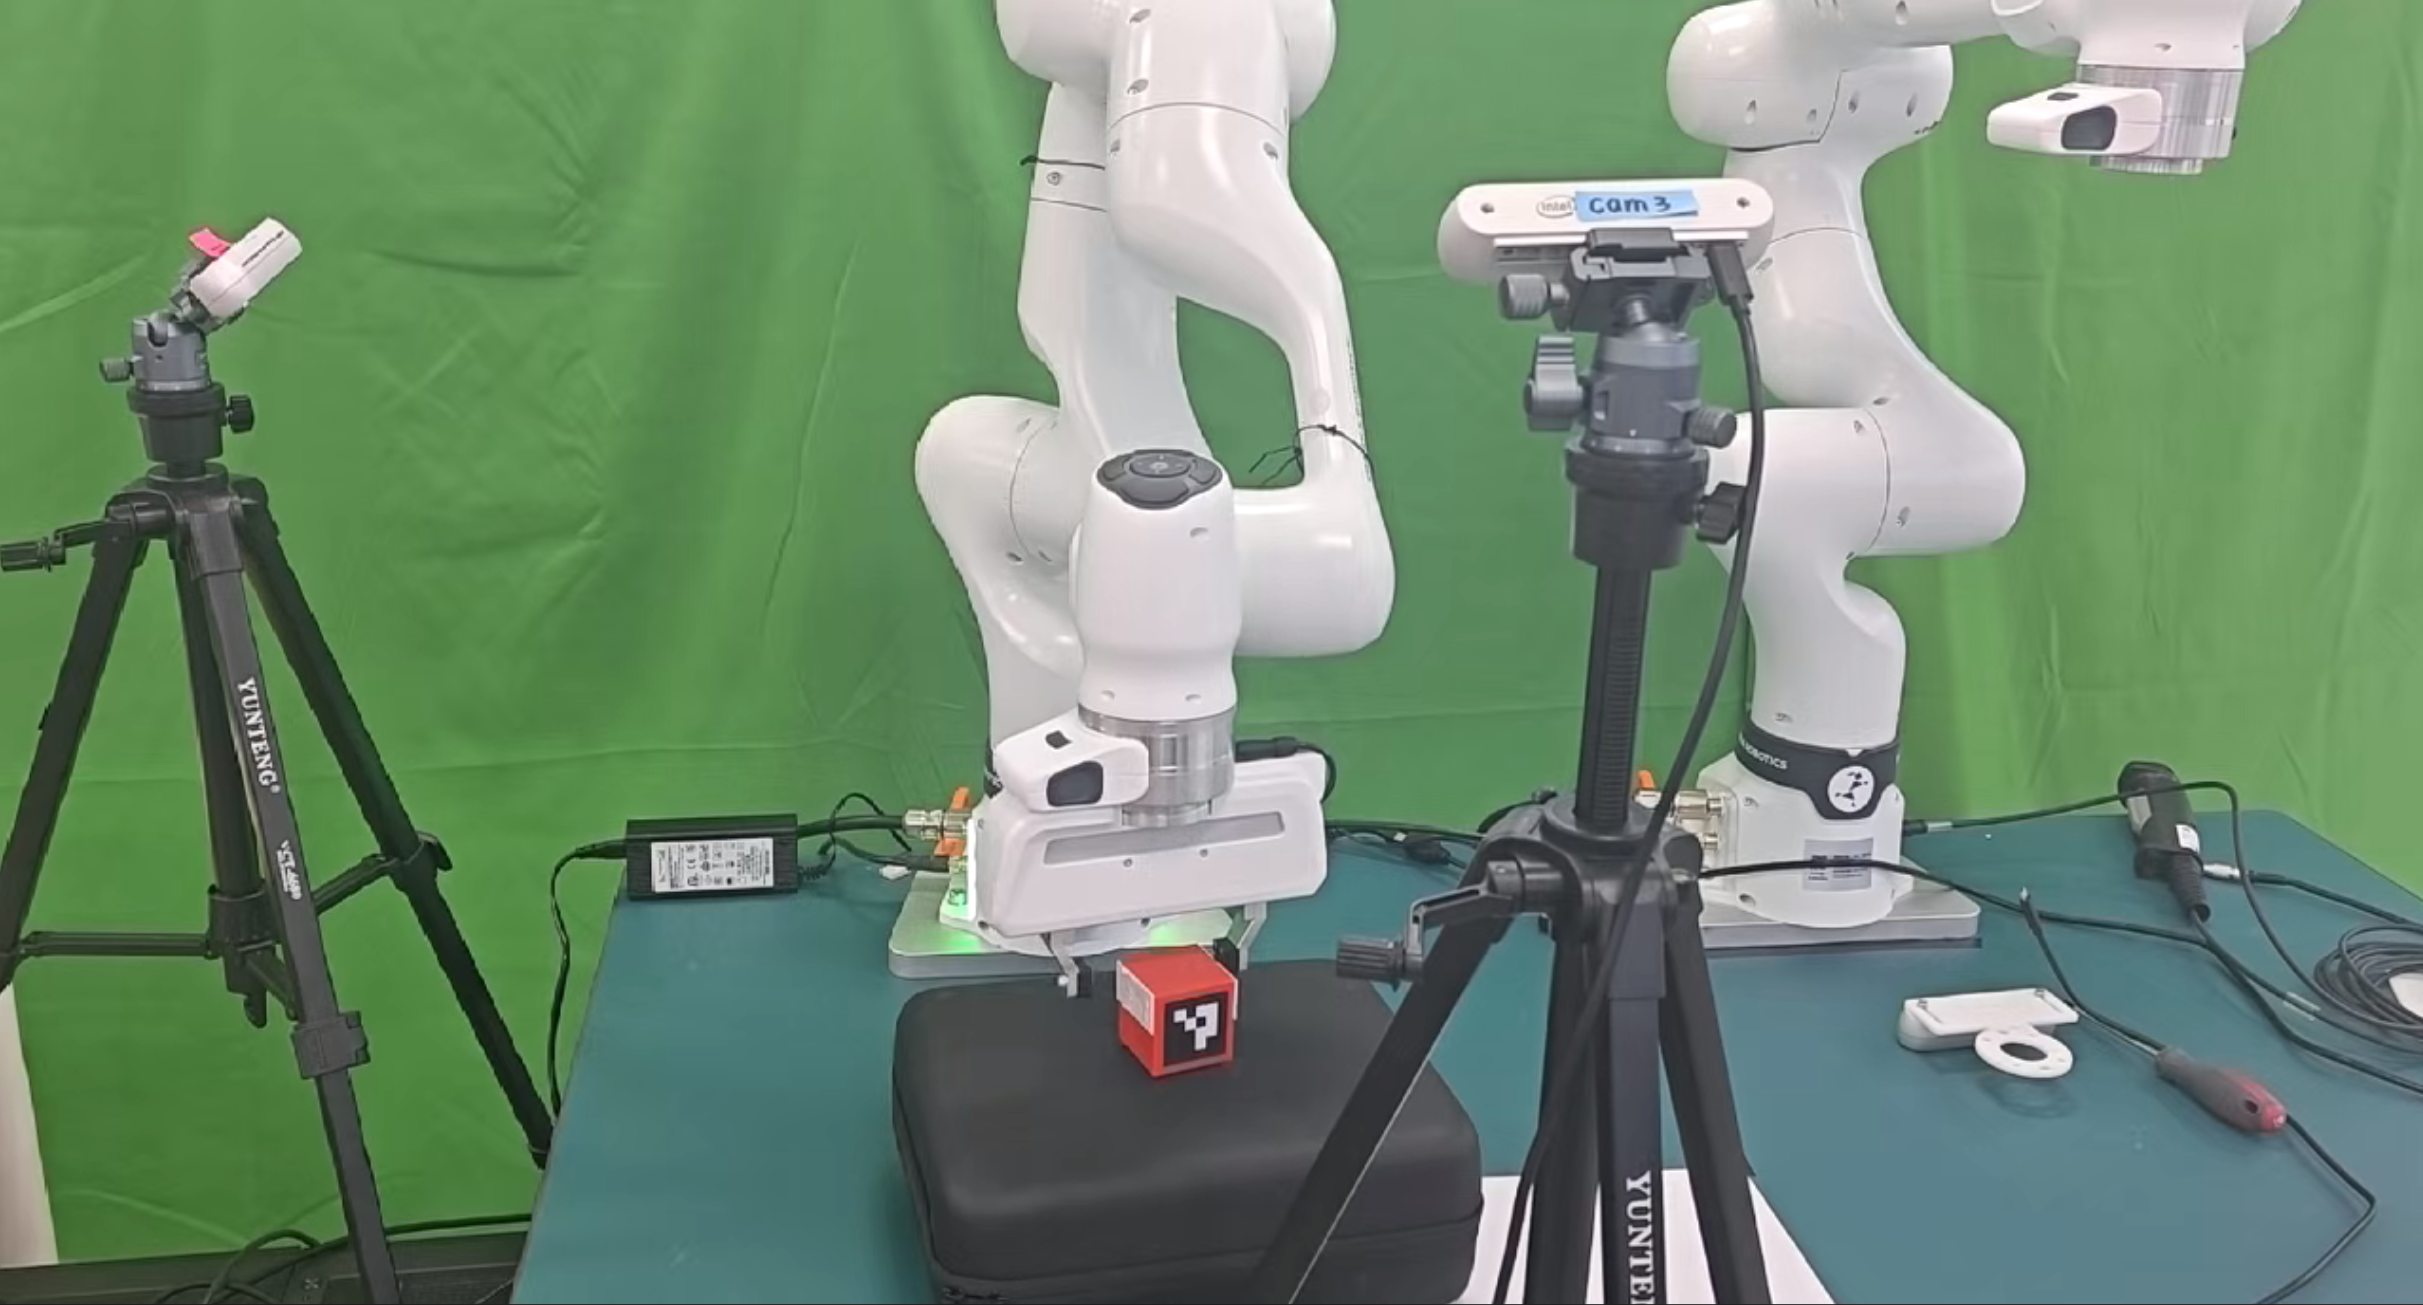
\includegraphics[width=\textwidth]{5.png}
        \caption{接近目标}
    \end{subfigure}

    \vspace{0.5em}

    \begin{subfigure}[b]{0.45\textwidth}
        \centering
        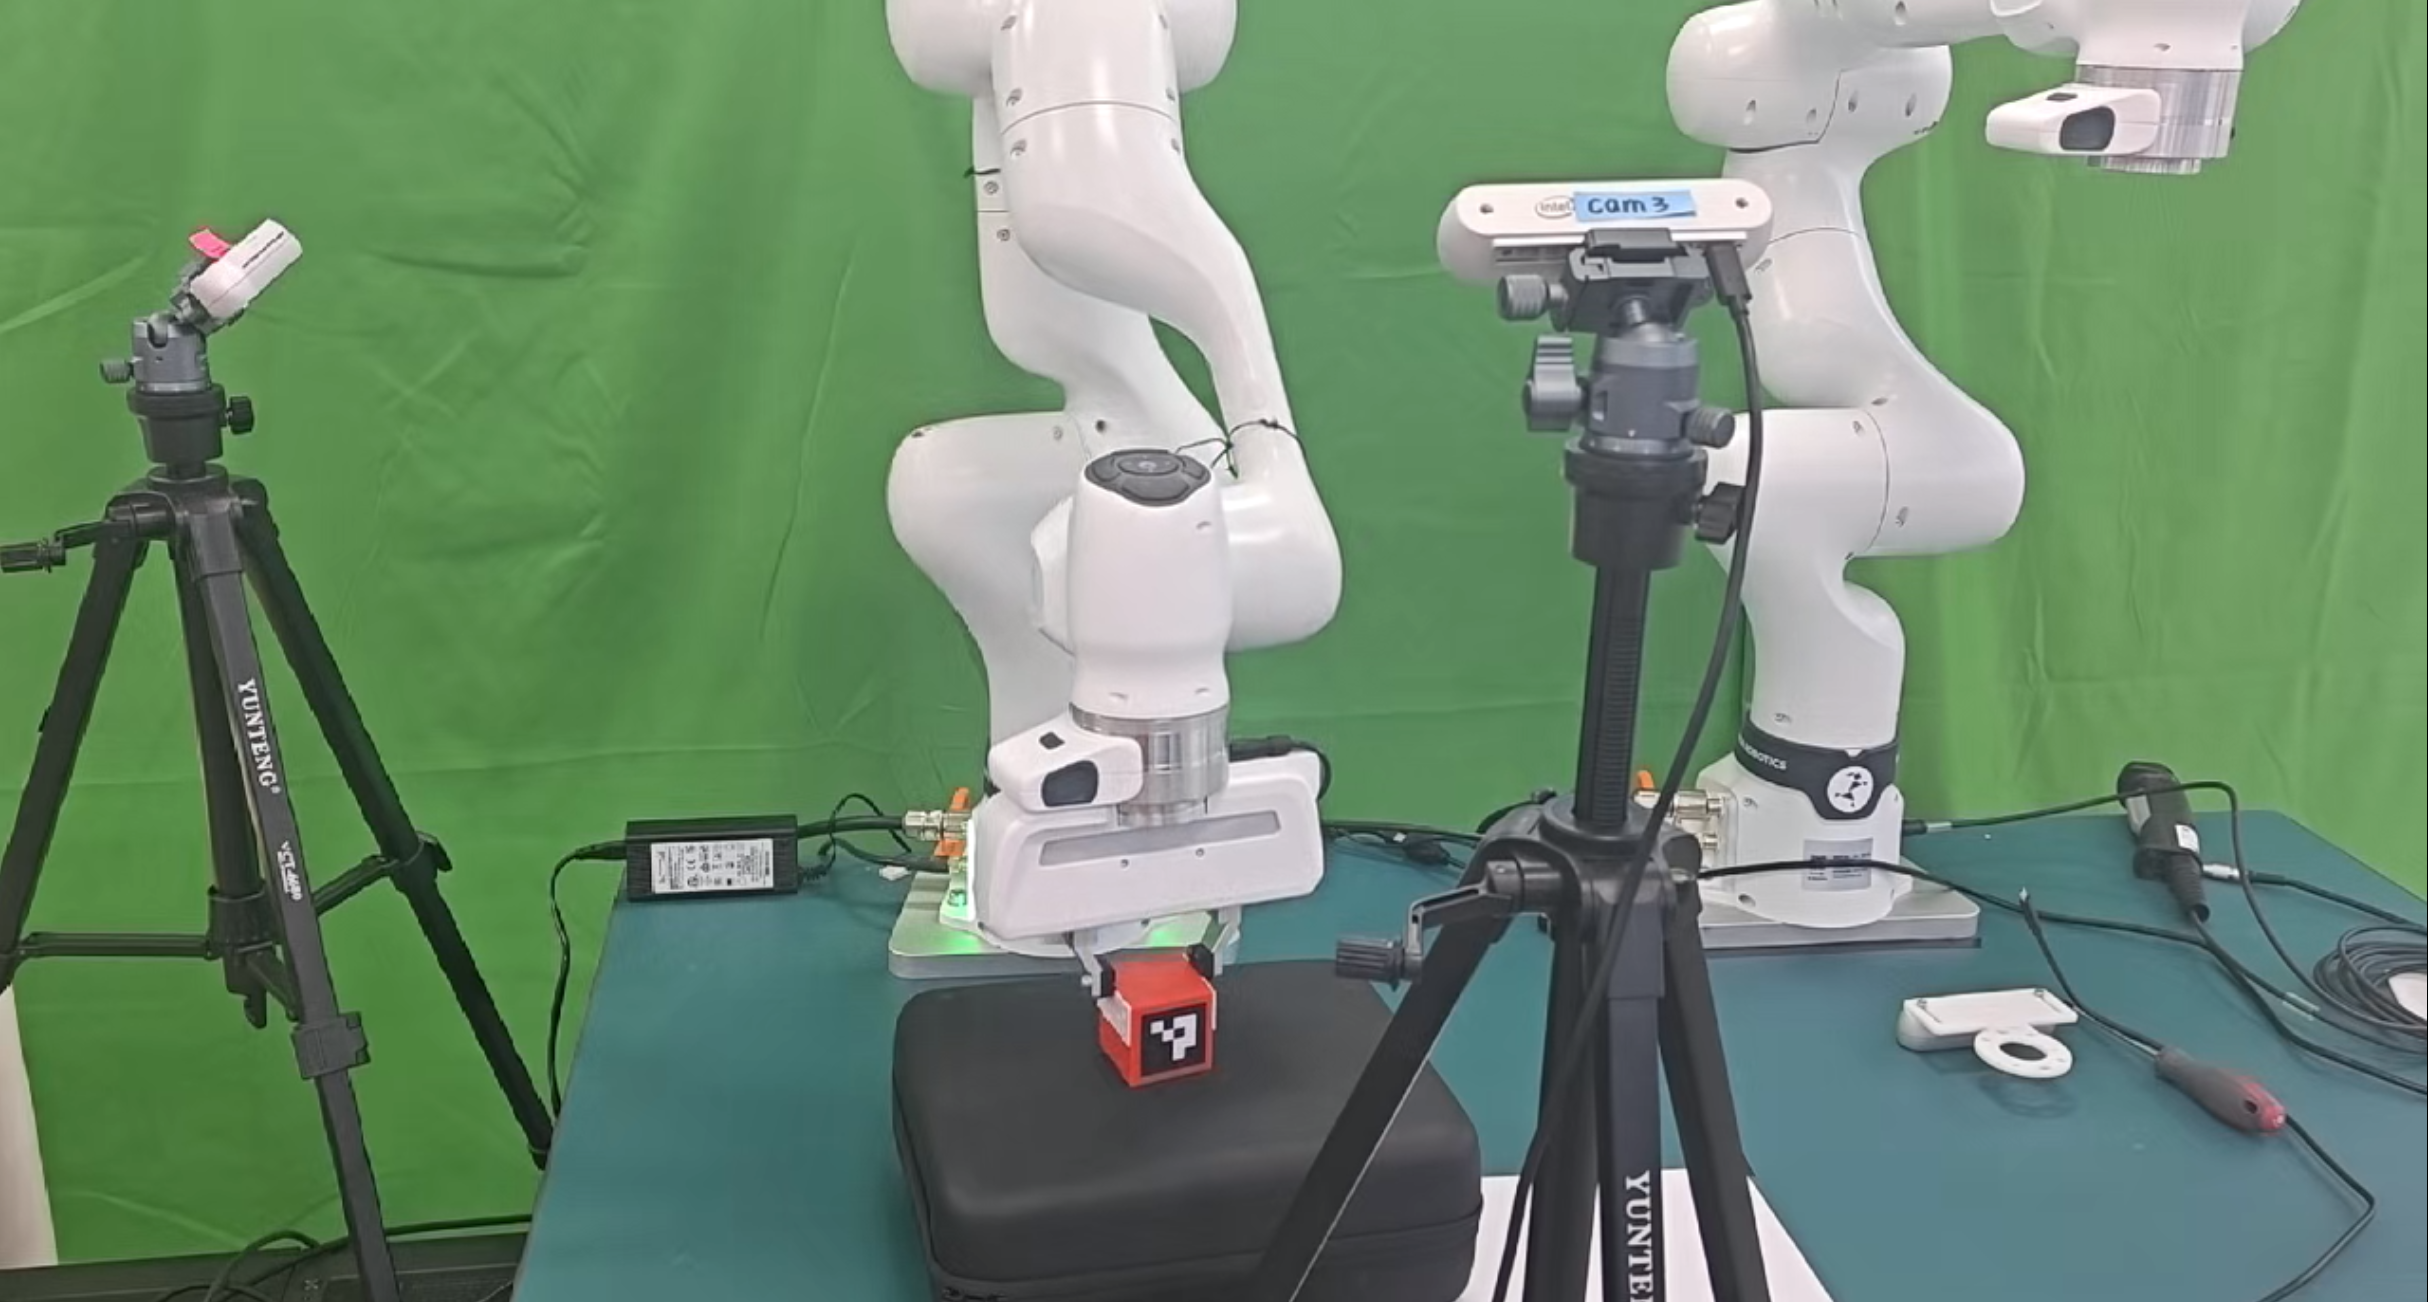
\includegraphics[width=\textwidth]{6.png}
        \caption{完成抓取}
    \end{subfigure}
    \hfill
    \begin{subfigure}[b]{0.45\textwidth}
        \centering
        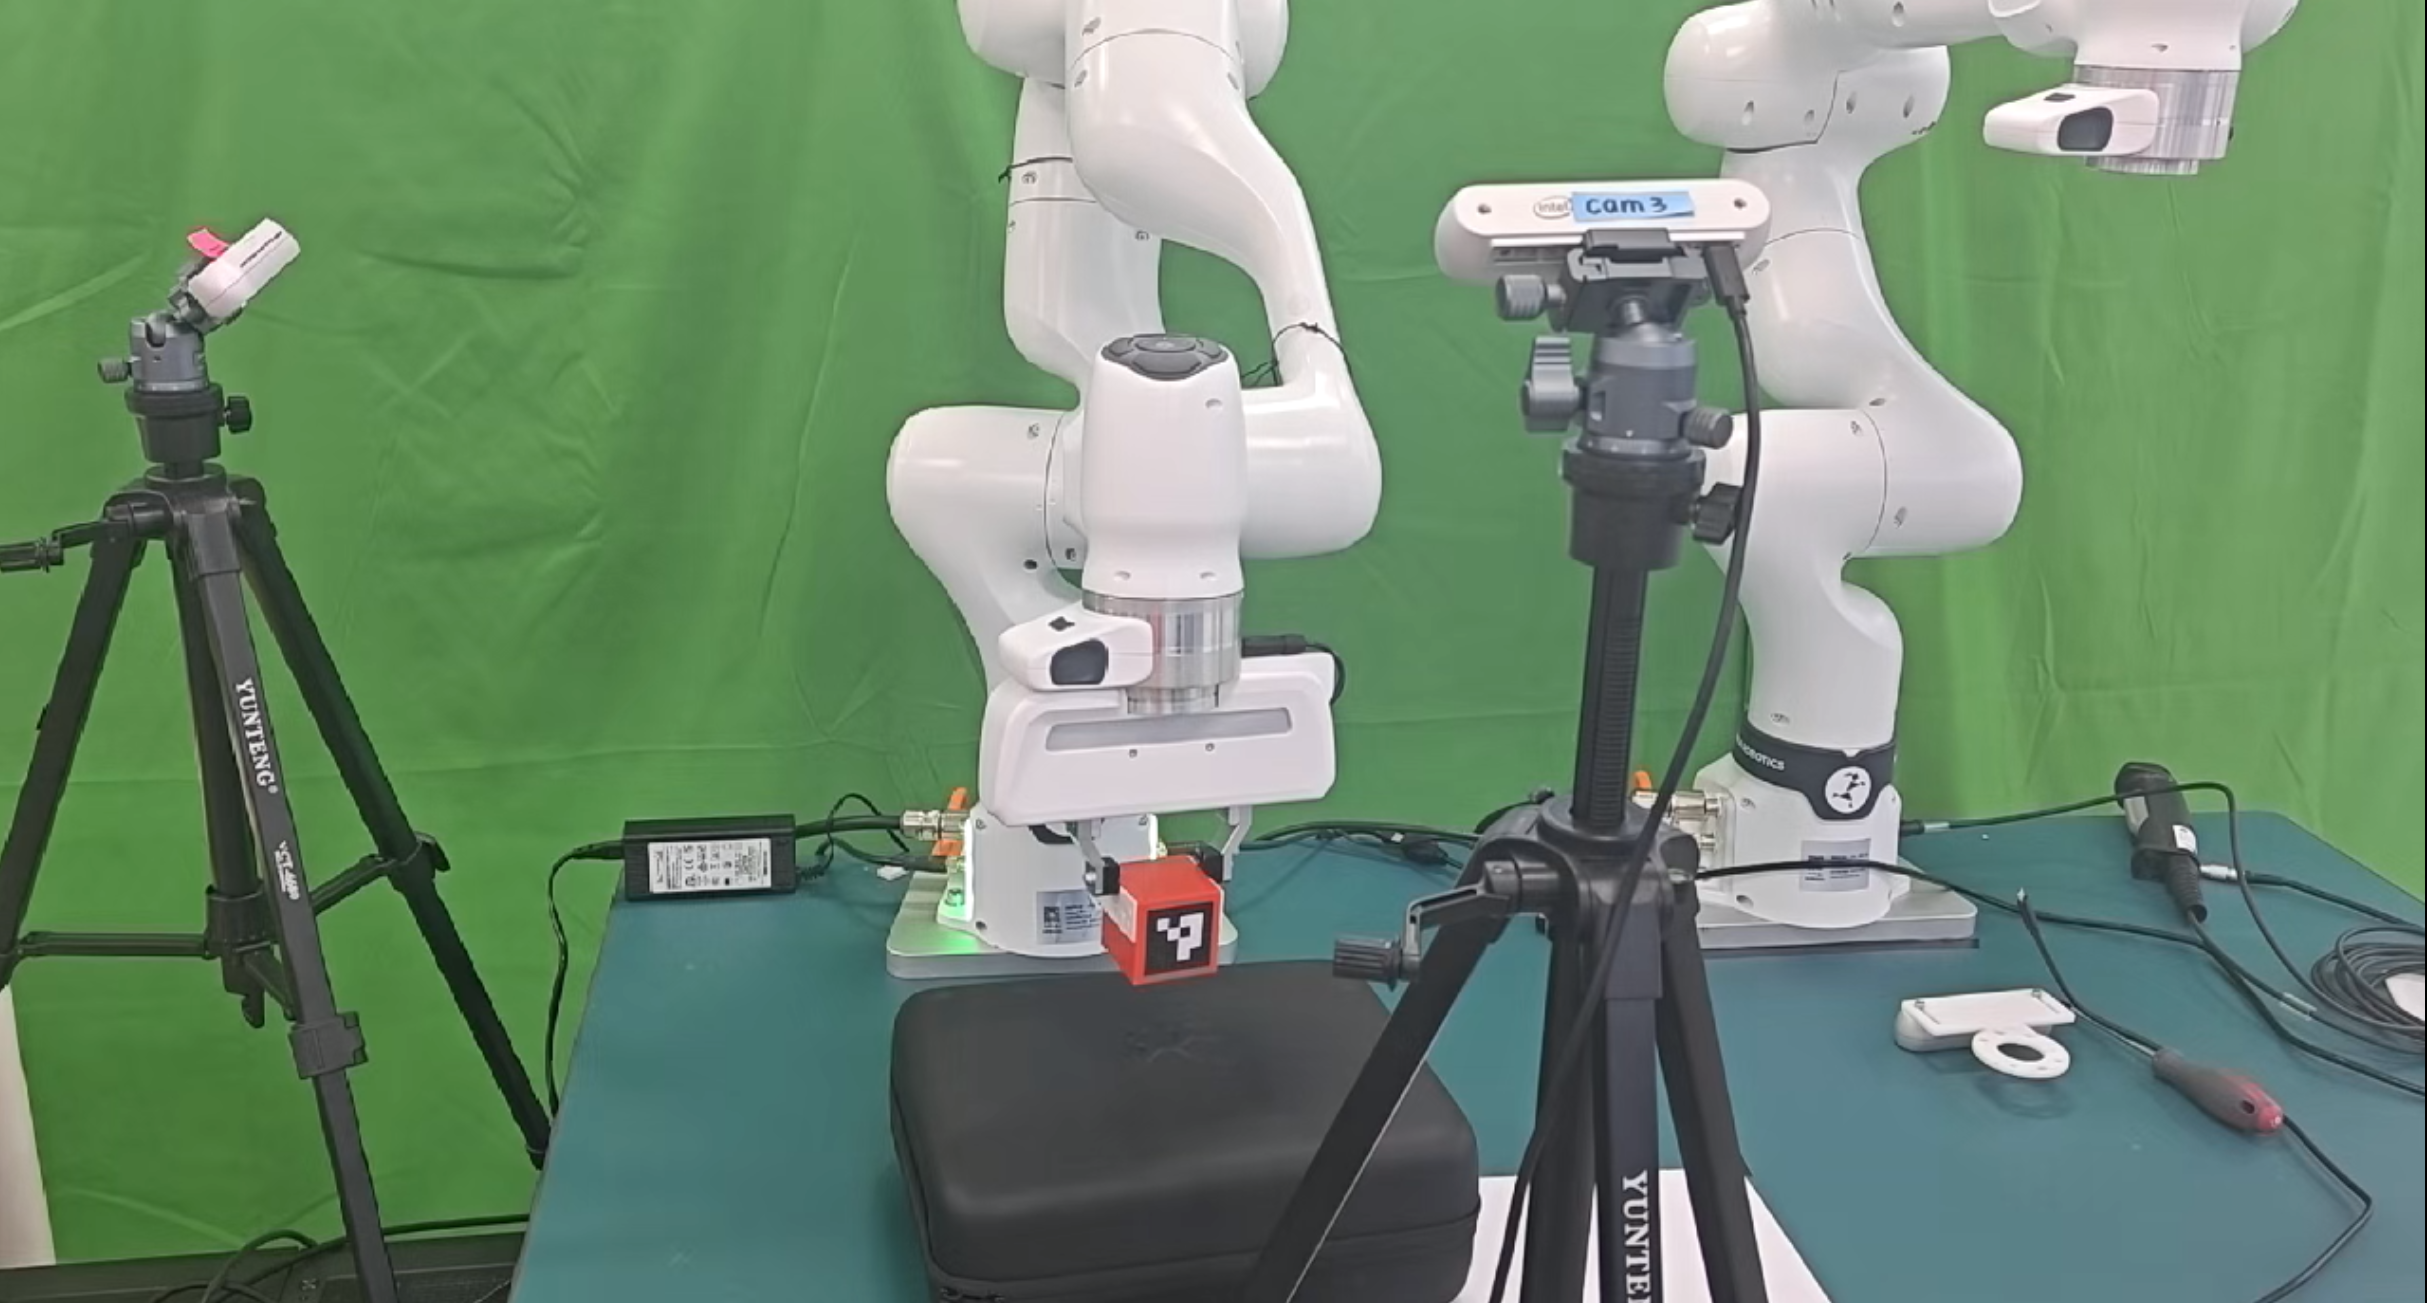
\includegraphics[width=\textwidth]{7.png}
        \caption{抬升且稳定保持}
    \end{subfigure}

    \caption{Franka Research 3 真实平台上的立方体抬升验证}
    \label{fig:real-fr3-sim-to-real-photo}
\end{figure}

从图\ref{fig:real-fr3-sim-to-real-photo}可以看出，机械臂能够根据视觉检测到的立方体位置逐步接近目标，并在靠近物体后由策略输出的夹爪动作触发闭合。夹爪闭合后，机械臂执行竖直抬升，立方体随夹爪离开桌面，说明仿真训练得到的策略在真实机械臂上完成了基本的抓取和抬升验证。该结果表明，使用机器人基坐标系构造观测、使用 ArUco 提供物体位姿、并将归一化策略动作转换为受限笛卡尔位移，是一条可行的低维策略 sim-to-real 路线。

真实实验也暴露出一些值得进一步改进的问题。首先，视觉检测的立方体位置存在轻微抖动，会导致策略输出在接近阶段发生小幅变化。其次，真实控制链路中 MoveIt 2 规划和执行存在一定延迟，使真实动作频率低于仿真环境。再次，夹爪闭合时机完全由策略第四维动作决定，如果视觉估计误差较大，仍可能出现提前闭合或偏心抓取。因此，后续可以进一步加入视觉滤波、夹爪接触检测、力反馈和更多次重复实验，以提升真机验证的稳定性和统计可靠性。

\section{安全措施}

真实机器人实验中，本文没有让强化学习策略直接输出关节力矩，而是采用“策略输出低频末端增量，控制器执行受限笛卡尔运动”的方式。程序中设置了工作空间边界、单步最大位移、最低接近高度、夹爪使能开关和人工停止机制。实验开始前先进行 shadow mode 测试，即只打印策略动作而不发送机器人命令；确认动作方向和坐标系一致后，再以较小速度进入真实执行模式。这些安全措施降低了策略从仿真迁移到真实平台时的风险。

\chapter{总结与展望}

\section{全文总结}

本文围绕“基于强化学习的机械臂操作算法研究”这一主题，基于 MuJoCo 和 robosuite 搭建了机械臂桌面立方体抬升任务环境，并使用 SAC 算法训练连续控制策略。本文设计了低维状态空间和操作空间位置动作空间，使策略能够学习末端运动和夹爪控制。针对初始策略中出现的过度上抬和随机摆动问题，本文提出了稳定抬升目标、工作空间约束、动作裁剪、运动惩罚和连续稳定保持成功判据。

实验分析表明，原始成功率只能反映物体是否被抬离桌面，不能准确评价策略是否稳定。通过引入 raw\_lift\_success\_rate、controlled\_lift\_success\_rate 和 held\_success\_rate 三类指标，可以更细致地分析策略行为。本文最终将 held\_success\_rate 作为主要任务指标，使训练目标更接近真实机械臂应用中“抬起并稳定保持”的需求。

在真实平台验证方面，本文进一步将仿真训练得到的策略部署到 Franka Research 3 机械臂上进行初步 sim-to-real 实验。真实系统通过 RealSense 相机和 ArUco 标记获取立方体位姿，并利用手眼标定将相机坐标系下的物体位姿转换到机器人基坐标系下，从而构造与仿真训练一致的低维观测。真实执行阶段采用受限的笛卡尔线性控制方式，将策略输出的归一化动作转换为小幅度末端位移，并结合夹爪动作完成接近、夹取和抬升。实验结果说明，在坐标系统一、动作限幅和安全约束的基础上，本文训练得到的低维位姿策略能够完成从仿真到真实机械臂的初步迁移验证。

\section{不足与展望}

本文仍存在一些不足。首先，当前策略使用低维状态输入，真实部署阶段依赖 ArUco 标记提供物体位姿，尚未实现无标记的通用视觉识别。其次，实验任务相对简单，只包含单个立方体的抬升操作，尚未扩展到多物体抓取、放置或装配任务。最后，本文已经完成 Franka Research 3 上的初步 sim-to-real 验证，但真实实验次数有限，尚未进行大规模重复实验、扰动实验和统计显著性分析。

后续工作可以从以下方向展开：
\begin{enumerate}
  \item 引入更通用的视觉感知模块，减少对 ArUco 标记和人工标定流程的依赖；
  \item 使用域随机化提升策略对真实环境差异的鲁棒性；
  \item 将任务扩展到 pick-and-place、堆叠和插孔等更复杂操作；
  \item 完善真实 Franka Research 3 控制包装器，加入力反馈、接触检测和失败恢复机制；
  \item 结合模仿学习和强化学习，使用人工示教提高训练效率。
\end{enumerate}

总体而言，本文完成了一个较完整的机械臂强化学习操作算法实验流程，并通过稳定保持指标改进了策略评价方式，同时完成了基于 Franka Research 3 的初步 sim-to-real 验证，为后续真实机械臂部署和更复杂操作任务研究奠定了基础。

\printbibliography

\begin{acknowledgement}
在本论文完成过程中，感谢指导老师邴老师在研究方向、实验设计和论文写作方面给予的指导。从论文选题、开题报告、系统设计到论文撰写，老师都给予了我悉心的指导和帮助。感谢姚相同博士、孟远博士、王博师兄、王宇轩同学和贾豪睿同学等所有在毕业论文中曾经帮助过我的师兄和同学。感谢开源社区提供的 MuJoCo、robosuite 和 Stable-Baselines3 等工具，使本文能够在较完整的机器人仿真平台上开展实验。
\end{acknowledgement}

\appendix

\chapter{系统模块说明}

本文实验系统由仿真环境模块、环境接口包装模块、强化学习训练模块、评价与日志模块、真实视觉定位模块以及真实机器人执行模块组成。各模块职责如下：

\begin{itemize}
  \item 仿真环境模块：负责加载机械臂、夹爪、桌面和立方体模型，并提供物理仿真、接触计算和原始奖励。
  \item 环境接口包装模块：负责将原始环境观测整理为低维状态向量，并将策略输出的归一化动作转换为可执行的末端位移和夹爪动作。
  \item 强化学习训练模块：负责使用 SAC 算法进行策略优化，保存训练过程中的最优策略模型和最终策略模型。
  \item 评价与日志模块：负责记录训练奖励、回合长度、原始抬升成功率、受控抬升成功率和稳定保持成功率，并生成实验曲线。
  \item 真实视觉定位模块：负责通过 RealSense 相机和 ArUco 标记估计立方体位姿，并结合手眼标定结果将物体位姿转换到机器人基坐标系。
  \item 真实机器人执行模块：负责构造真实观测、加载训练后的策略模型、执行动作限幅和工作空间裁剪，并通过笛卡尔线性控制接口驱动 Franka Research 3 完成接近、夹取和抬升。
\end{itemize}

\end{document}
